% !TEX root = ./iclr2026_conference.tex


\section{Introduction}
Mathematical optimization is one of the pillars of modern machine learning (ML), equipping us with the numerical tools needed to compute parameters for large-scale decision systems. In this work, we focus on \emph{variational inequality problems (VIPs)} \citep{stampacchia1964formes}—a unifying framework that extends beyond classical loss minimization to encompass min–max optimization, complementarity problems \citep{dantzig1968complementary,facchinei2003finite}, equilibrium computation in games, and general fixed-point formulations  \citep{bauschke2017convex}. In recent years, VIPs have gained significant traction in ML and data science, especially due to their broad potential applicability in domains where minimizing a single empirical loss is insufficient, with notable examples including generative adversarial networks \citep{goodfellow2014generative,arjovsky2017wasserstein}, multi-agent and robust reinforcement learning \citep{namkoong2016stochastic,wang2021adversarial,giannou2022convergence}, and auction theory \citep{syrgkanis2015fast}.

In practice, many of these tasks reduce to finite-sum formulations, where the objective depends on a large collection of data samples or agents. In such settings, \emph{stochastic gradient methods} have become the workhorse of large-scale learning \citep{bottou2018optimization}. By exploiting the finite-sum structure, stochastic gradient descent (SGD) and its variants replace expensive full-gradient computations with inexpensive updates on a few components, enabling scalability to massive datasets. 

While the theoretical underpinnings of SGD have been extensively studied \citep{rakhlin2011making,raginsky2017non,azizian2024long,MalickMertikopoulos2024}, much of its practical success can be traced to a handful of seemingly “low-level” heuristics \citep{bottou2012stochastic}: step-size schedules (constant vs.\ decaying), data ordering (with vs.\ without resampling), and iterate selection (average vs.\ last iterate). To facilitate analysis, the community has typically adopted a \emph{ceteris paribus} perspective—isolating one design choice at a time while holding the rest fixed—an approach that clarifies individual effects but obscures their interaction.

A particularly important case is the use of a \emph{constant step size} {\color{blue}$\gamma$, which is popular in practice because it simplifies tuning, it quickly erases dependence on initialization, and it yields fast early progress \citep{yu2021analysis}. However, its fundamental drawback is that convergence halts at a non-vanishing error.} Even in strongly convex problems with unique solution $x^*$, the last iterate of SGD typically satisfies: \[\text{$\text{MSE}(\texttt{SGD})=\limsup_{k\to\infty}\ex[\|x_k-x^*\|^2]=\mathcal{O}(\gamma)$ and $\text{bias}(\texttt{SGD})=\limsup_{k\to\infty}\|\ex[x_k]-x^*\|=\mathcal{O}(\gamma)$.}\] Thus, the iterates stabilize in the long run at distance from the optimum on the order of the step size.

%Even in the simple case of strongly convex problems with a unique solution $x^*$, one typically has
%\(
%\limsup_{k\to \infty} |\ex[x_k]-x_*|\leq  C e^{-\rho k} +\text{bias}(\gamma)
%%\exof{\mathrm{dist}^2(x_k, x_*)}=
%%%x_k = x_*+ 
%%e^{-\rho k}\exof{\mathrm{dist}^2(x_0, x_*)} + \text{resid}(\gamma),
%\)
%where the first term decays exponentially while the residual satisfies $\text{bias}(\gamma) = \mathcal{O}(\gamma)$. Thus, in the long run, the iterates stabilize at a point whose distance from the optimum remains on the order of the step size.
%
%To address this issue, practitioners often turn to debiasing heuristics. One such technique, widely adopted in stochastic optimization, is \emph{random reshuffling} (\RRresh), or \emph{without-replacement} sampling, where each data point is used exactly once per epoch. Unlike classical \emph{with-replacement} SGD, which may revisit or skip samples, \RRresh\ enforces a random full pass that mirrors practical large-scale training \citep{bottou2018optimization}. Despite the dependence it induces across samples, recent work has established faster convergence guarantees for \RRresh\ in both minimization \citep{ahn2020sgd,gurbuzbalaban2021random,cai2023empirical} and VIPs \citep{mishchenko2020revisiting,emmanouilidis2024stochastic}, along with sharper \emph{MSE} bounds from $\mathcal{O}(\gamma)$ to $\mathcal{O}(\gamma^2)$ under suitable conditions.
%
%
%To mitigate this limitation, practitioners often employ debiasing heuristics. A prominent example is \emph{random reshuffling} (\RRresh), or \emph{without-replacement} sampling, where each data point is visited exactly once per epoch. Unlike classical \emph{with-replacement} SGD, which may resample or skip points, \RRresh\ enforces a random full pass that closely mirrors large-scale training in practice \citep{bottou2018optimization}. Although it induces dependence across samples, recent work has established faster convergence guarantees for \RRresh\ in both minimization \citep{ahn2020sgd,gurbuzbalaban2021random,cai2023empirical} and VIPs \citep{mishchenko2020revisiting,emmanouilidis2024stochastic}, along with sharper \emph{MSE} bounds—improving from $\mathcal{O}(\gamma)$ to $\mathcal{O}(\gamma^2)$ under suitable conditions.
%

$\blacktriangleright$To mitigate this limitation, practitioners often turn to debiasing heuristics.  A prominent example is \emph{random reshuffling} (\RRresh), or \emph{without-replacement} sampling, where each data point is visited exactly once per epoch. Unlike classical \emph{with-replacement} SGD, which may resample or skip points, \RRresh\ enforces a random full pass that closely mirrors large-scale training in practice \citep{bottou2018optimization}. Despite the dependence it induces across samples, recent work has established faster convergence guarantees for \RRresh\ in both minimization \citep{ahn2020sgd,gurbuzbalaban2021random,cai2023empirical} and VIPs \citep{mishchenko2020revisiting,emmanouilidis2024stochastic}, along with sharper \emph{MSE} bounds from $\mathcal{O}(\gamma)$ to $\mathcal{O}(\gamma^2)$.
{\color{blue}However, the question of whether the bias term itself improves has remained open.}
%, while leaving open the question of whether the bias term itself improves. 
Indeed, recall that for any estimator $\hat x$, the mean squared error decomposes as
\[
\mathrm{MSE}(\hat x) \;=\; \ex[\|\hat x - x^*\|^2] \;=\; \|\ex[\hat x]-x^*\|^2 \;+\; \mathrm{Var}(\hat x),
\]
so that $\mathrm{bias}(\hat x) \le \sqrt{\mathrm{MSE}(\hat x)}$. Under this trivial bound, \textsc{SGD–\RRresh} guarantees improved MSE compared to vanilla SGD, but does not necessarily yield smaller bias.


$\blacktriangleright$ Orthogonal to reshuffling, another classical idea from numerical analysis has recently re-emerged in stochastic optimization: \emph{\citeauthor{richardson1911ix}–\citeauthor{romberg1955vereinfachte}} (\RRrom) \emph{extrapolation}. Its principle is simple yet powerful: \emph{Run the algorithm of your choice with two different step sizes and combine their outputs so that the leading bias term cancels.} Concretely, whenever the bias admits an expansion of the form $\text{bias}(\gamma) = \Delta \gamma + \mathcal{O}(\gamma^{\kappa})$ with $\kappa>1$, running the stochastic approximation at two step sizes gives:
\vspace{-0.25em}\[\text{$x_{\infty}^{\gamma} - x^* = \Delta \gamma + \mathcal{O}(\gamma^{\kappa})$ and $x_{\infty}^{2\gamma} - x^* = 2\Delta \gamma + \mathcal{O}(\gamma^{\kappa})$.}\vspace{-0.25em}\] 
Extrapolating these iterates then yields: \vspace{-0.25em} 
\[
x_{\text{extr}}- x^*
= 2x_{\infty}^{\gamma} - x_{\infty}^{2\gamma} - x^*
= \cancel{2\Delta \gamma} - \cancel{2\Delta \gamma} + \mathcal{O}(\gamma^{\kappa})
= \mathcal{O}(\gamma^{\kappa}). \vspace{-0.25em}
\]
Originally introduced for accelerating discretization schemes in stochastic differential equations \citep{hildebrand1987introduction,talay1990expansion,bally1996law}, \RRrom\ has since been applied to optimization, improving constant-step methods from SGD \citep{durmus2016stochastic,dieuleveut2020bridging,mangold2024refined,sheshukova2024nonasymptotic} to Q-learning and two-timescale stochastic approximation methods \citep{huo2023bias,kwon2024two,zhang2024constant,allmeier2024computing}. {\color{red}Despite} its conceptual simplicity and empirical success, its theoretical foundations for stochastic VIPs remain nascent \citep{vlatakis2024stochastic}. 
\kostas{Even though it remains conceptually simple and empirically successful, its theoretical foundations for stochastic VIPs remain nascent \citep{vlatakis2024stochastic}.}

{\color{red}Despite} this progress, the known \emph{bias} rates of the heuristics remain limited {\color{blue}only when they are applied separately.}
For unconstrained strongly monotone VIPs, \RRrom\ alone attains $\mathcal{O}(\gamma^{3/2})$ bias \citep{vlatakis2024stochastic}\footnote{The $\mathcal{O}(\gamma^2)$ rate in \citet[Sec.~5, Thm.~6]{vlatakis2024stochastic} is obtained via a reduction to \citet[Sec.~3, Thm.~4]{dieuleveut2020bridging}, which requires additional noise assumptions not met in our setting.}, 
whereas \RRresh\ is known to sharpen \emph{MSE} bounds (from $\mathcal{O}(\gamma)$ to $\mathcal{O}(\gamma^2)$) but does not, in general, guarantee an improved bias order.
\kostas{However, it remains unclear whether one can combine effectively the aforementioned heuristics in a unified method that outperforms both. This raises the natural question:} 
{\color{blue}This raises a natural question: can one synthesize these approaches into a unified framework that outperforms both,
}
%This raises a natural challenge: can one synthesize the two so as to surpass both, 
ideally reaching $\mathcal{O}(\gamma^{3})$ bias?
\begin{equation}
\parbox{35em}{\centering
\textit{What new phenomena arise when these heuristics\\—
\emph{constant step sizes, random reshuffling, and Richardson extrapolation}—\\
interact simultaneously?}
}
\tag{$\bigstar$}
\label{central-question}
\end{equation}
{\color{red}I don't like putting one question inline, the other in star. Just say it rises two questions and state one after the other inline.}
%
%Despite the aforementioned progress, the asymptotic bias rates of the two heuristics remain limited when applied in isolation. 
%For unconstrained strongly monotone VIPs, it is known that \RRrom\ alone achieves order $\mathcal{O}(\gamma^{1.5})$ \citep{vlatakis2024stochastic}
%\footnote{The $\mathcal{O}(\gamma^2)$ rate in \citet[Sec.~5, Thm.~6]{vlatakis2024stochastic} is obtained via a reduction to the framework of \citet[Sec.~3, Thm.~4]{dieuleveut2020bridging}, but that reduction requires additional noise assumptions not satisfied in our setting.}
%%\footnote{In the analysis of \citet{vlatakis2024stochastic}, the $\mathcal{O}(\gamma^2)$ rate is obtained by reduction to the framework of \citet{dieuleveut2020bridging}; however, the latter requires additional noise assumptions that are not satisfied by the stochastic structure of the problem.}
%, while \RRresh\ reaches $\mathcal{O}(\gamma^{2})$
%\citep{emmanouilidis2024stochastic}.
% Thus, the tantalizing prospect is to combine these two heuristics in a principled way to reach $\mathcal{O}(\gamma^{3})$.%, even though the known lower bound remains $\mathcal{O}(\gamma^{2})$. 
%This naturally raises the central question of our work:
%%Thus, the optimal scenario is to realize the composition of these two improvements, achieving $\mathcal{O}(\gamma^{3})$, while the lower bound remains at $\mathcal{O}(\gamma^{2})$. 
%%This raises a fundamental question: 
%%This is precisely the question 
%%This raises a fundamental question that we establish in this work:
%\begin{equation}
%\parbox{35em}{\centering
%\textit{What new phenomena arise when these heuristics\\—
%\emph{constant step sizes, random reshuffling, and Richardson extrapolation }—\\
%interact simultaneously? }
%}
%\tag{$\bigstar$}
%\label{central-question}
%\end{equation}
%Addressing this question is non-trivial: \RRresh\ produces a biased stochastic oracle whose discrete noise structure lies outside the scope of existing analyses for mainly unbiased \RRrom\ methods \citep{dieuleveut2020bridging,sheshukova2024nonasymptotic,vlatakis2024stochastic}. \\\\
Addressing this question is delicate. Reshuffling introduces a biased stochastic oracle whose discrete, permutation-driven noise structure lies outside the reach of existing analyses of extrapolation, which predominantly assume unbiased or continuously distributed perturbations \citep{dieuleveut2020bridging,sheshukova2024nonasymptotic,vlatakis2024stochastic}.\\

% \vspace{-0.75em}\textbf{Our model's assumptions.}
% While variational inequalities provide a unifying language for optimization, learning, and game dynamics, \emph{no single structural assumption can capture the full complexity of all modern nonconvex--nonconcave problems}. From a computational standpoint, even smooth VIs are intractable in full generality---being tightly connected to Nash equilibria~\citep{
% papadimitriou2022computational,goldberg2022ppad}, linear complementarity~\citep{ieor2011linear}, and constrained saddle-point problems~\citep{daskalakis2021complexity}. Consequently, much of the theoretical literature adopts \emph{structured} assumptions (strong convexity, quasi-strong monotonicity, quasar or weak convexity, PL/KL conditions, Minty conditions, error bounds, etc.), each expressive in specific regimes but not universal.

% Our work is based on \emph{quasi-strong monotonicity} which falls squarely within this class: it captures stabilizing behaviors of many smooth systems, while remaining far more permissive than strong convexity or global monotonicity. At the same time, it is helpful to clarify that this assumption is not meant as a universal model for all adversarial or fully nonconvex--nonconcave settings. Certain modern ML applications---
% including GANs, adversarial robustness, and multi-agent RL---can exhibit fundamentally unstable or rotational dynamics~\citep{Jin2020LocalOptimality,Han2023RiemannianMinimax,KimSeo2022SemiImplicit,Bukharin2023RobustMARL}, where even \emph{local} monotonicity surrogates fail. As such, our theoretical guarantees should be viewed as pertaining to regimes where a minimum amount of local structure is present, rather than to the most adversarial or unstructured cases.
% \footnote{A complementary and key fact for our setting, established in \citep[Lemma~A.4]{hsieh2019convergence}, is that \emph{any smooth VI operator is locally quasi-strongly monotone in a neighborhood of a regular solution}. Combined with our Markov-chain recurrence result—which ensures that the iterates remain in such neighborhoods with probability~1—this provides a natural and widely adopted stability regime in which the $\RRresh$ and $\RRrom$ debiasing mechanisms are both theoretically justified and practically meaningful.
% }

% {\color{red}I don't get the point of the first two paragraphs. The first one, rather than stating our model assumptions, is a review of others. Then the second goes in many directions. Why not just jumpt to the contributions and state the assumptions in there. The details can go in the main body.}

% {\color{orange}Manolis: Send the above two paragraphs in a appendix}

\textbf{Our contributions.}
Motivated by this gap, we undertake in this work what is, to the best of our knowledge, the first systematic study demonstrating that these heuristics can be synthesized into a principled algorithmic framework.
%, yielding a composite bias reduction unattainable by any of them in isolation. 
Our main result shows that their composition yields a level of bias reduction unattainable by either heuristic alone. 
To this end, we extend and refine previous analyses of both \RRresh\ and \RRrom, and we introduce a novel algorithm (Algorithm~\ref{alg:rrrom-rrresh}) that achieves their optimal composition without requiring any additional assumptions:
\vspace{+0.15cm}
\begin{maininformal}
For quasi-strongly monotone smooth VIPs, our combined method (SGD-\RRrom$\oplus$\RRresh, Algorithm~\ref{alg:rrrom-rrresh}) cancels all lower-order terms in the bias expansion, yielding an asymptotic bias of order $\mathcal{O}(\gamma^3)$.
\end{maininformal}

% \kostas{I think we can skip the sentence on the model assumptions in order to have better connection with the next paragraph.} 
% {\color{orange}Manolis: Write one sentence that for concision we present the discussion about the adopted our model assumption (e.g. quasi-storng monotonicity) in Appendix X}

To establish the above result, we first derive an intermediate finding: in isolation, \texttt{Perturbed SGD-\RRresh} achieves an asymptotic bias of $C\gamma+\mathcal{O}(\gamma^3)$—to the best of our knowledge, the first analysis of its kind. This is particularly striking: although without-replacement sampling induces a biased gradient estimator, it paradoxically yields an improved bias rate (see Figure~\ref{fig:biases}).\begin{wrapfigure}{r}{0.45\linewidth}
    \centering
    \includegraphics[width=0.75\linewidth]{./figures/relative_error_plots/new_plot_manolis_gamma_0.0001_condition_num_1.pdf}
    \caption{\small
    Illustration of bias behavior. 
    Example on a min–max quadratic VIP with 
    $F(x,y)=\tfrac{1}{N}\sum_{i\in[N]} x^\top A_i x + x^\top B_i y + y^\top C_i y$ 
    for $N=1000$, where $A_i,B_i,C_i$ are quasi–strongly monotone. 
    Already after the second epoch batch, the methods clearly separate: 
    \textcolor{blue}{SGD}, \textcolor{orange}{\RRresh}, 
    \textcolor{darkgreen}{\RRrom}, and 
    \textcolor{red}{\RRresh$\oplus$\RRrom}. 
    }
    \vspace{-1.5em}
    \label{fig:biases}
\end{wrapfigure}

% \textbf{Comparison to Prior Work and Overview of Our Contributions.}
% Before introducing the intuition behind our algorithmic design, we briefly contrast our results with those of \cite{emmanouilidis2024stochastic}, who study \RRresh-based improvements for the Stochastic Extragradient (SEG) method. 
% Our analysis uncovers a fundamentally different phenomenon: the joint use of $\RRresh \oplus \RRrom$ produces a \emph{bias cancellation mechanism} that eliminates the leading $\mathcal{O}(\gamma)$ term while preserving the condition number and asymptotic behavior of SGDA. 
% The key distinctions are summarized in Table~\ref{tab:comparison}. 
% Achieving the best of both worlds—optimal bias order together with a tight condition number, as SEG without reshuffling enjoys—remains an interesting direction for future work.

% % \vspace{-0.35cm}

% \begin{table}[h!]
% \centering
% \scalebox{0.92}{
% \footnotesize
% \begin{tabular}{lcc}
% \toprule
% \textbf{Aspect} & \textbf{\cite{emmanouilidis2024stochastic}} & \textbf{Our work} \\
% \midrule

% Baseline Algorithm & \textbf{SEG} & \textbf{SGDA} \\[2pt]

% Model Assumptions (Smoothness) &
% $F_i$--$L_i$ Lipschitz &
% $F_i$--$L_i$ Lipschitz
% \\[2pt]

% Model Assumptions (Drift) &
% $F$ $\mu$--strongly monotone &
% $F$ \emph{quasi}--strongly monotone
% \\[2pt]

% Main heuristic & \textbf{\RRresh\ only} & \textbf{\RRresh\ $\oplus$ \RRrom} \\[2pt]

% Asymptotic Bias order & $\mathcal{O}(\gamma + \gamma^3)$ & $\mathcal{O}(\gamma^3)$ \\[2pt]

% Asymptotic MSE order & $\mathcal{O}(\gamma^2)$ & $\mathcal{O}(\gamma^2)$ \\[2pt]

% Condition number & \textbf{Worse than vanilla-SEG} & \textbf{Same as vanilla-SGDA} \\[2pt]

% Mechanism & EG-structure + $\RRresh$ & Bias cancellation ($\RRresh \oplus \RRrom$) \\
% \bottomrule
% \end{tabular}
% } % end scalebox
% \caption{Summary of key differences between Emmanouilidis--Vidal--Loizou (2024) and our results.}
% \label{tab:comparison}
% \end{table}
% \vspace{-2em}

% \newpage
% {\color{red}
% \textbf{Comparison to Prior Work and Overview of Our Contributions}
% Before presenting the high level intuition of our algorithm, we provide a concise comparison between our results and the recent work of \cite{emmanouilidis2024stochastic}, which analyzes \RRresh-based improvements for the Stochastic Extragradient (SEG) method. Our findings reveal a qualitatively different behavior: by combining \emph{two} complementary reshuffling operators (RR$_1$ and RR$_2$), we demonstrate a systematic \textit{bias cancellation mechanism} that preserves the favorable statistical properties of SGDA while eliminating the leading-order bias term. We summarize this contrast in Table~\ref{tab:comparison}, which highlights the conceptual and technical distinctions between the two approaches.
% ---<Λιγο πιο μαζεμενο κειμενο
% {---< Βαλε καποιο scalebox
% \begin{table}[h!]
% \centering
% \caption{Summary of key differences between Emmanouilidis--Vidal--Loizou (2024) and our results.}
% \label{tab:comparison}
% \begin{tabular}{lcc}
% \toprule
% \textbf{Aspect} & \textbf{\cite{emmanouilidis2024stochastic}} & \textbf{Our work} \\
% \midrule
% Baseline Algorithm & \textbf{SEG} & \textbf{SGDA} \\[2pt]
% <--- Fix this lineModel Assumptions & $F_i$-L_i Lipischtz and $F$-$\mu$ strongly monotone & $F_i$-L_i Lipischtz and $F$-$\mu$ quasi strongly monotone \\[2pt]
% Main heuristic & \textbf{\RRresh only} & \textbf{\RRresh $\oplus$ \RRrom} \\[2pt]
% Asymptotic Bias order & $\mathcal{O}(\gamma + \gamma^3)$ & $\mathcal{O}(\gamma^3)$ \\[2pt]
% Asymptotic MSE order & $\mathcal{O}(\gamma^2)$ & $\mathcal{O}(\gamma^2)$ \\[2pt]
% Condition number & \textbf{Worse than vanilla-SEG} & \textbf{Same as vanilla-SGDA} \\[2pt]
% Mechanism & EG-structure + $\RRresh$ & Bias cancellation ($\RRresh \oplus \RRrom$) \\
% \bottomrule
% \end{tabular}
% \end{table}

% Our analysis shows that the interaction of $RR_1$ and $RR_2$ is not a cosmetic modification but a structural phenomenon: the two reshuffling layers eliminate the linear-order bias term and yield an estimator whose behavior matches the ``ideal'' SGDA dynamics in expectation. This provides the first principled explanation of why SGDA--RR can enjoy both \emph{faster transient regimes} and \emph{unimpaired asymptotic variance}, without relying on the extragradient correction or restrictive smoothness assumptions.}


%\newpage
%
%
%Originally introduced for accelerating discretization schemes in stochastic differential equations \citep{hildebrand1987introduction,talay1990expansion,bally1996law}, \RRrom\ has since found applications across optimization, improving constant-step methods from SGD \citep{durmus2016stochastic,dieuleveut2020bridging,mangold2024refined,sheshukova2024nonasymptotic} to Q-learning and two-timescale stochastic approximation \citep{huo2023bias,kwon2024two,zhang2024constant,allmeier2024computing}. Despite its conceptual simplicity and empirical success, its theoretical underpinnings for stochastic VIPs remain underdeveloped \citep{vlatakis2024stochastic}. 
%
%Yet, the bias reduction achieved by \RRrom\ and by \RRresh\ is fundamentally limited when each is applied in isolation. For unconstrained strongly monotone VIPs, it is known that \RRrom\ alone achieves order $\mathcal{O}(\gamma^{1.5})$ \citep{vlatakis2024stochastic}\footnote{The $\mathcal{O}(\gamma^2)$ rate in \citet{vlatakis2024stochastic} is obtained via reduction to the framework of \citet{dieuleveut2020bridging}, but this requires additional noise assumptions not satisfied in our setting.}, while \RRresh\ attains $\mathcal{O}(\gamma^{2})$ \citep{emmanouilidis2024stochastic}. Thus, the tantalizing prospect is to combine these two heuristics in a principled way to reach $\mathcal{O}(\gamma^{3})$, even though the known lower bound remains $\mathcal{O}(\gamma^{2})$. 
%
%This naturally raises the central question:
%\begin{equation}
%\parbox{35em}{\centering
%\textit{What new phenomena arise when these heuristics---\\
%\emph{constant step sizes, random reshuffling, and Richardson extrapolation}---\\
%are brought to interact simultaneously?}
%}
%\tag{$\bigstar$}
%\label{central-question}
%\end{equation}
%
%Addressing this question is delicate. Random reshuffling introduces a biased stochastic oracle whose discrete, permutation-driven noise structure lies outside the reach of existing analyses of \RRrom, which predominantly assume unbiased or continuously distributed perturbations \citep{dieuleveut2020bridging,sheshukova2024nonasymptotic,vlatakis2024stochastic}.
%
%\subsection{Our Contributions.}
%
%Motivated by this gap, we provide, to the best of our knowledge, the first systematic analysis demonstrating that these heuristics can indeed be synthesized into a unified algorithmic framework. Our main result shows that their composition yields a level of bias reduction unattainable by either heuristic alone. To this end, we refine the analyses of both \RRresh\ and \RRrom, and we introduce a novel algorithm (Algorithm~\ref{alg:rrrom-rrresh}) that achieves their optimal composition without requiring additional assumptions:
%
%\begin{maininformal}
%For quasi-strongly monotone smooth VIPs, our combined method (\RRrom$\oplus$\RRresh, Algorithm~\ref{alg:rrrom-rrresh}) cancels all lower-order terms in the bias expansion, achieving an asymptotic bias of order $\mathcal{O}(\gamma^3)$.
%\end{maininformal}

% \begin{figure}[ht]\label{fig:biases}
% %\vspace{-2em}
%     \centering
%     % Left image
%     \begin{minipage}{0.48\linewidth}
%         \centering
%           \includegraphics[width=0.7\linewidth]{./figures/relative_error_plots/new_plot_manolis_gamma_0.0001_condition_num_1.pdf.pdf}
% %        \includegraphics[width=0.8\linewidth]{./placeholder.pdf}
%         %\caption*{(a) Bias trajectories for a toy VIP example.}
%     \end{minipage}
%     \hfill
%     % Right image
%     \begin{minipage}{0.48\linewidth}
%         \centering
%         \scalebox{0.345}{% !TEX root = ./iclr2026_conference.tex

\tikzset{every picture/.style={line width=0.75pt}}        

\begin{tikzpicture}[x=0.75pt,y=0.75pt,yscale=-1,xscale=1]


%Shape: Ellipse [id:dp7329906304802944] 
\draw  [fill={rgb, 255:red, 74; green, 144; blue, 226 }  ,fill opacity=0.29 ] (481.22,393.5) .. controls (481.22,299.89) and (557.06,224) .. (650.61,224) .. controls (744.16,224) and (820,299.89) .. (820,393.5) .. controls (820,487.11) and (744.16,563) .. (650.61,563) .. controls (557.06,563) and (481.22,487.11) .. (481.22,393.5) -- cycle ;
%Shape: Ellipse [id:dp14673386188875415] 
\draw  [fill={rgb, 255:red, 126; green, 211; blue, 33 }  ,fill opacity=0.41 ] (537.7,393.5) .. controls (537.7,331.1) and (588.25,280.52) .. (650.61,280.52) .. controls (712.97,280.52) and (763.52,331.1) .. (763.52,393.5) .. controls (763.52,455.9) and (712.97,506.48) .. (650.61,506.48) .. controls (588.25,506.48) and (537.7,455.9) .. (537.7,393.5) -- cycle ;
%Shape: Ellipse [id:dp3138874134344609] 
\draw  [fill={rgb, 255:red, 245; green, 166; blue, 35 }  ,fill opacity=1 ] (568.79,393.5) .. controls (568.79,348.28) and (605.42,311.62) .. (650.61,311.62) .. controls (695.8,311.62) and (732.44,348.28) .. (732.44,393.5) .. controls (732.44,438.72) and (695.8,475.38) .. (650.61,475.38) .. controls (605.42,475.38) and (568.79,438.72) .. (568.79,393.5) -- cycle ;
%Shape: Ellipse [id:dp6951380714624634] 
\draw  [fill={rgb, 255:red, 208; green, 2; blue, 27 }  ,fill opacity=0.73 ] (617.47,393.5) .. controls (617.47,375.18) and (632.31,360.34) .. (650.61,360.34) .. controls (668.91,360.34) and (683.75,375.18) .. (683.75,393.5) .. controls (683.75,411.82) and (668.91,426.66) .. (650.61,426.66) .. controls (632.31,426.66) and (617.47,411.82) .. (617.47,393.5) -- cycle ;

% =============== COLORED POLYLINES WITH STARS ===============

% Green path
\draw [color={rgb, 255:red, 110; green, 192; blue, 19 }, line width=2.25]
  (356,490) -- (341,370) -- (418,243) -- (508,191) -- (594,212) -- (626.22,296.33);
\foreach \p in {(356,490),(341,370),(418,243),(508,191),(594,212),(626.22,296.33)}{
  \node[star, star points=5, draw={rgb,255:red,110; green,192; blue,19},
        fill={rgb,255:red,110; green,192; blue,19}, minimum size=7pt, inner sep=0pt] at \p {};
}

% Blue path
\draw [color={rgb, 255:red, 74; green, 144; blue, 226 }, line width=2.25]
  (356,490) -- (321,336) -- (362,258) -- (424,199) -- (499,157) -- (607,151)
  -- (698,178) -- (728,218) -- (713.68,258.29);
\foreach \p in {  (356,490) , (321,336) , (362,258) , (424,199) , (499,157) , (607,151)
  , (698,178) , (728,218) , (713.68,258.29)}{
  \node[star, star points=5, draw={rgb,255:red,74; green,144; blue,226},
        fill={rgb,255:red,74; green,144; blue,226}, minimum size=7pt, inner sep=0pt] at \p {};
}

% Orange path
\draw [color={rgb, 255:red, 206; green, 131; blue, 13 }, line width=2.25]
  (356,490) -- (388,387) -- (498,266) -- (574,267) -- (601,279) -- (618.6,339.2);
\foreach \p in {(356,490),(388,387),(498,266),(574,267),(601,279),(618.6,339.2)}{
  \node[star, star points=5, draw={rgb,255:red,206; green,131; blue,13},
        fill={rgb,255:red,206; green,131; blue,13}, minimum size=7pt, inner sep=0pt] at \p {};
}

% Red path
\draw [color={rgb, 255:red, 165; green, 6; blue, 24 }, line width=2.25]
  (356,490) -- (420,388) -- (504,346) -- (580,343) -- (641.61,376.61);
\foreach \p in {(356,490),(420,388),(504,346),(580,343),(641.61,376.61)}{
  \node[star, star points=5, draw={rgb,255:red,165; green,6; blue,24},
        fill={rgb,255:red,165; green,6; blue,24}, minimum size=7pt, inner sep=0pt] at \p {};
}

% =============================================================
%
%% Text Node
%\draw (632.38,393.8) node [anchor=north west][inner sep=0.75pt]  [font=\Large,color={rgb, 255:red, 255; green, 255; blue, 255 }  ,opacity=1 ]  {$x_{*}$};
%% Text Node
%\draw (606.03,200.22) node [anchor=north west][inner sep=0.75pt]  [font=\Large,color={rgb, 255:red, 74; green, 144; blue, 226 }  ,opacity=1 ,rotate=-0.45]  {$\mathrm{bias}( \gamma ) =\ \mathcal{O}\left( \gamma \right)$};
%% Text Node
%\draw (671.93,254.71) node [anchor=north west][inner sep=0.75pt]  [font=\Large,color={rgb, 255:red, 100; green, 172; blue, 43 },opacity=1 ,rotate=-25.81]  {$\mathrm{bias}( \gamma ) =\ \mathcal{O}\left( \gamma ^{1.5}\right)$};
%% Text Node
%\draw (598.56,429.08) node [anchor=north west][inner sep=0.75pt]  [font=\Large,color={rgb, 255:red, 208; green, 2; blue, 27 }  ,opacity=1 ,rotate=-0.61]  {$\mathrm{bias}( \gamma ) =\ \mathcal{O}\left( \gamma ^{3}\right)$};
%% Text Node
%\draw (720.43,309.21) node [anchor=north west][inner sep=0.75pt]  [font=\large,color={rgb, 255:red, 231; green, 151; blue, 19 }  ,opacity=1 ,rotate=-60.58]  {$\mathrm{bias}( \gamma ) =\ \mathcal{O}\left( \gamma ^{2}\right)$};
%% Text Node
%\draw (372.38,478.8) node [anchor=north west][inner sep=0.75pt]  [font=\Large,color={rgb, 255:red, 0; green, 0; blue, 0 }  ,opacity=1 ]  {$x_{0}$};

% Text Node
\draw (632.38,393.8) node [anchor=north west][inner sep=0.75pt]  [font=\Large,color={rgb, 255:red, 255; green, 255; blue, 255 }  ,opacity=1 ]  {$x_{*}$};
% Text Node
\draw (606.03,200.22) node [anchor=north west][inner sep=0.75pt]  [font=\large,color={rgb, 255:red, 74; green, 144; blue, 226 }  ,opacity=1 ,rotate=-0.45]  {$\mathrm{bias}( \gamma ) =\ O( \gamma )$};
% Text Node
\draw (665.93,244.71) node [anchor=north west][inner sep=0.75pt]  [font=\large,color={rgb, 255:red, 83; green, 146; blue, 2 }  ,opacity=1 ,rotate=-25.81]  {$\mathrm{bias}( \gamma ) =\ O\left( \gamma ^{1.5}\right)$};
% Text Node
\draw (595.56,429.08) node [anchor=north west][inner sep=0.75pt]  [font=\large,color={rgb, 255:red, 208; green, 2; blue, 27 }  ,opacity=1 ,rotate=-0.61]  {$\mathrm{bias}( \gamma ) =\ O\left( \gamma ^{3}\right)$};
% Text Node
\draw (716.43,301.21) node [anchor=north west][inner sep=0.75pt]  [font=\normalsize,color={rgb, 255:red, 180; green, 117; blue, 0 }  ,opacity=1 ,rotate=-60.58]  {$\mathrm{bias}( \gamma ) =\ O\left( \gamma ^{2}\right)$};
% Text Node
\draw (365.38,478.8) node [anchor=north west][inner sep=0.75pt]  [font=\LARGE,color={rgb, 255:red, 0; green, 0; blue, 0 }  ,opacity=1 ]  {$x_{0}$};

%Straight Lines [id:da7873343135782715] 
\draw    (650.61,393.5) -- (648.05,234) ;
\draw [shift={(648,231)}, rotate = 89.08] [fill={rgb, 255:red, 0; green, 0; blue, 0 }  ][line width=0.08]  [draw opacity=0] (10.72,-5.15) -- (0,0) -- (10.72,5.15) -- (7.12,0) -- cycle    ;
\draw [shift={(650.61,393.5)}, rotate = 269.08] [color={rgb, 255:red, 0; green, 0; blue, 0 }  ][fill={rgb, 255:red, 0; green, 0; blue, 0 }  ][line width=0.75]      (0, 0) circle [x radius= 3.35, y radius= 3.35]   ;
%Straight Lines [id:da8747548930371518] 
\draw    (650.61,393.5) -- (695.72,297.71) ;
\draw [shift={(697,295)}, rotate = 115.22] [fill={rgb, 255:red, 0; green, 0; blue, 0 }  ][line width=0.08]  [draw opacity=0] (10.72,-5.15) -- (0,0) -- (10.72,5.15) -- (7.12,0) -- cycle    ;
\draw [shift={(650.61,393.5)}, rotate = 295.22] [color={rgb, 255:red, 0; green, 0; blue, 0 }  ][fill={rgb, 255:red, 0; green, 0; blue, 0 }  ][line width=0.75]      (0, 0) circle [x radius= 3.35, y radius= 3.35]   ;
%Straight Lines [id:da18150789044644122] 
\draw    (650.61,393.5) -- (713.61,347.16) ;
\draw [shift={(716.03,345.38)}, rotate = 143.66] [fill={rgb, 255:red, 0; green, 0; blue, 0 }  ][line width=0.08]  [draw opacity=0] (10.72,-5.15) -- (0,0) -- (10.72,5.15) -- (7.12,0) -- cycle    ;
\draw [shift={(650.61,393.5)}, rotate = 323.66] [color={rgb, 255:red, 0; green, 0; blue, 0 }  ][fill={rgb, 255:red, 0; green, 0; blue, 0 }  ][line width=0.75]      (0, 0) circle [x radius= 3.35, y radius= 3.35]   ;
%Straight Lines [id:da6863210759512379] 
\draw    (650.61,393.5) -- (665.12,418.22) ;
\draw [shift={(666.64,420.81)}, rotate = 239.59] [fill={rgb, 255:red, 0; green, 0; blue, 0 }  ][line width=0.08]  [draw opacity=0] (10.72,-5.15) -- (0,0) -- (10.72,5.15) -- (7.12,0) -- cycle    ;
\draw [shift={(650.61,393.5)}, rotate = 59.59] [color={rgb, 255:red, 0; green, 0; blue, 0 }  ][fill={rgb, 255:red, 0; green, 0; blue, 0 }  ][line width=0.75]      (0, 0) circle [x radius= 3.35, y radius= 3.35]   ;



% % Central point and labels
% \draw (632.38,393.8) node [anchor=north west][inner sep=0.75pt] [font=\large,color=white] {$x_{*}$};
% \draw (606.03,200.22) node [anchor=north west][font=\footnotesize,color={rgb, 255:red, 74; green, 144; blue, 226 }] {$\mathrm{bias}( \gamma ) =\ O( \gamma )$};
% \draw (671.93,254.71) node [anchor=north west][font=\footnotesize,color={rgb, 255:red, 126; green, 211; blue, 33 }] {$\mathrm{bias}( \gamma ) =\ O\!\left( \gamma ^{1.5}\right)$};
% \draw (598.56,429.08) node [anchor=north west][font=\footnotesize,color={rgb, 255:red, 208; green, 2; blue, 27 }] {$\mathrm{bias}( \gamma ) =\ O\!\left( \gamma ^{3}\right)$};
% \draw (720.43,309.21) node [anchor=north west][font=\footnotesize,color={rgb, 255:red, 231; green, 151; blue, 19 }] {$\mathrm{bias}( \gamma ) =\ O\!\left( \gamma ^{2}\right)$};
% \draw (372.38,478.8) node [anchor=north west][font=\large,color=black] {$x_{0}$};

\end{tikzpicture}}
%         %\caption*{(b) Asymptotic neighborhood of $x_k$.}
%     \end{minipage}
%     \vspace{-1em}
%     \caption{\small
%     Illustration of bias behavior. 
%     \textbf{(a) Left:} Example on a min–max quadratic VIP with 
%     $F(x,y)=\tfrac{1}{N}\sum_{i\in[N]} x^\top A_i x + x^\top B_i y + y^\top C_i y$ 
%     for $N=1000$, where $A_i,B_i,C_i$ are quasi–strongly monotone. 
%     Already after the second epoch batch, the methods clearly separate: 
%     \textcolor{blue}{SGD}, \textcolor{orange}{\RRresh}, 
%     \textcolor{darkgreen}{\RRrom}, and 
%     \textcolor{red}{\RRresh$\oplus$\RRrom}. 
% \textbf{(b) Right:} Concentric regions around $x^*$ depict the asymptotic neighborhoods determined by the bias term. 
% %in the decomposition $|\ex[x_k- x_*]|= C e^{-k} + \text{bias}_{\text{method}}(\gamma)$. 
% Colored trajectories show the different rates: 
% (\textcolor{blue}{SGD}, $\mathcal{O}(\gamma)$), 
% (\textcolor{darkgreen}{\RRrom}, $\mathcal{O}(\gamma^{1.5})$), 
% (\textcolor{orange}{\RRresh}, $\mathcal{O}(\gamma^{2})$), 
% and 
% (\textcolor{red}{\RRresh$\oplus$\RRrom}, $\mathcal{O}(\gamma^{3})$). 
%     \vspace{-1.em}}
% \end{figure}



%We believe that our framework offers a principled design paradigm that extends naturally to other constant step-size stochastic methods—ranging from single-call to multi-call extragradient schemes, and encompassing extragradient, optimistic, and mirror-prox variants \citep{hsieh2019convergence, azizian2020tight}. We leave the full exploration of these directions to future work.\vspace{-0.5em}
% \paragraph{Our algorithm.}  
% While there are many conceivable ways to interleave \RRrom\ and \RRresh, both intra- and inter-epoch, we adopt the most natural and practically motivated design. In modern pipelines, \RRresh\ is the workhorse at the low-level training stage, while \RRrom\ is often employed as a black-box refinement at a higher level, allowing parallelization and modular integration.

% \begin{wrapfigure}{r}{0.45\linewidth}
%     \centering
%     \includegraphics[width=0.75\linewidth]{./figures/relative_error_plots/new_plot_manolis_gamma_0.0001_condition_num_1.pdf}
%     \caption{\small
%     Illustration of bias behavior. 
%     Example on a min–max quadratic VIP with 
%     $F(x,y)=\tfrac{1}{N}\sum_{i\in[N]} x^\top A_i x + x^\top B_i y + y^\top C_i y$ 
%     for $N=1000$, where $A_i,B_i,C_i$ are quasi–strongly monotone. 
%     Already after the second epoch batch, the methods clearly separate: 
%     \textcolor{blue}{SGD}, \textcolor{orange}{\RRresh}, 
%     \textcolor{darkgreen}{\RRrom}, and 
%     \textcolor{red}{\RRresh$\oplus$\RRrom}. 
%     }
%     \vspace{-1.5em}
%     \label{fig:biases}
% \end{wrapfigure}

% Accordingly, we study stochastic gradient algorithms that sample via random reshuffling to generate stochastic oracles of gradients/operators. At the start of each epoch $k>0$, a random permutation $\omega_k$ of $[n]$ is drawn, prescribing the order in which data points are processed. The algorithm then performs the classical SGD update:
% \begin{equation}\tag{SGD-\RRrom$\oplus$\RRresh (inner-loop)}
% \footnotesize
%     x_k^{i+1} = x_k^i - \gamma \,\mathrm{PreProcess}\big[\mathrm{StochOracle}(x^i_k; \omega_k^i)\big],
%     \label{SGD-4R1}
% \end{equation}

% where $\mathrm{StochOracle}(x^i_k; \omega_k^i)$ denotes either the stochastic gradient (in minimization problems) or the operator value $F_{\omega_k^i}(x^i_k)$ (in the general VI case), indexed by the $\omega_k^i$ data point and $\mathrm{PreProcess}[\cdot]$ is a preprocessing routine implementing calibrated Gaussian smoothing to the input. Then, the final iterate of each epoch becomes the starting point of the next, and the procedure repeats.
% %
% %A key difficulty stems from the biased nature of reshuffling: after one epoch, the cumulative estimator is a biased proxy of the finite-sum gradient.
% %This precisely motivates the widespread use of sampling with replacement, which is unbiased and analytically simpler. Moreover, the noise induced by reshuffling is inherently discrete, with support tied to the space of permutations. To address this, we introduce a preprocessing routine that smooths the discrete noise distribution into a well-behaved proxy, while preserving its variance and moment structure. We show that a carefully calibrated Gaussian perturbation suffices; however, for large datasets the effect is already negligible, indicating that preprocessing may ultimately be unnecessary. Understanding its precise dependence on dataset size remains an open direction for future work.

% \emph{On the necessity of smoothing.}
% A key challenge with reshuffling is that, after one epoch, the cumulative gradient estimator is biased, unlike sampling with replacement, which is unbiased and analytically simpler. The induced noise is also discrete, tied to permutations. 
% To handle this, we introduce a calibrated Gaussian perturbation that smooths the discrete reshuffling noise into a well-behaved proxy while preserving variance, moments, and bias order. In practice, the perturbation has negligible effect across datasets; clarifying its precise dependence on dataset size is an interesting direction for future work. For completeness, the supplement also includes a brief sketch showing how our results extend even without this step.

% Finally, at the end of each epoch we apply \RRrom, yielding the extrapolated update:
% \begin{equation}\tag{SGD-\RRrom$\oplus$\RRresh (outer-loop)}
%     \hat{x}^N_{I+1} = 2\,x^{N}_{I,[\gamma]} - x^{N}_{I,[2\gamma]}\,.
%     \label{SGD-4R2}
% \end{equation}
% In Section~\ref{sec:results}, we prove that this combination achieves a provable $\mathcal{O}(\gamma^3)$ bias— to the best of our knowledge, the first such result. There we also provide the detailed description of Algorithm~\ref{alg:rrrom-rrresh} together with the formal statement specifying its exact parameter choices.\vspace{-1em}
\paragraph{Proof outline and technical innovations.}
We now sketch the main ingredients of our analysis, deferring complete statements and proofs to Section~\ref{sec:results} and the appendix. 
As our optimization landscape, we consider variational inequality problems (VIPs) satisfying weak quasi-strong monotonicity, a class broad enough to cover many structured non-monotone and non-convex problems. 
Intuitively, quasi-strong monotonicity ensures a directional drift towards equilibrium, but unlike strong convexity it offers no uniform control. 
Its weak variant relaxes this further, introducing a systemic error that diminishes even this limited drift.  
Our roadmap proceeds through three main stations:

$\star$ \emph{Convergence of SGD-\RRresh\ under perturbations.}  
We first analyze the \RRresh\ component, proving exponential convergence with bias linear under weak and quadratic under quasi-strong monotonicity, robust even to preprocessing perturbations. 
We also derive higher-moment bounds of the form $\exof{\dist^p(x_k,x^*)}$ (Lemma~\ref{lemma strongly monotone 4th-moment}), which are essential for the bias decomposition required in the analysis of  \RRrom\ component
\footnote{Under quasi-strong monotonicity the VI has a unique solution. Under weak quasi-strong monotonicity, Theorem~\ref{thm: convergence_rate} applies to the \emph{projection} onto the solution set, as standard under Assumption~\ref{assumpt: weak_quasi_strong_monotonicity}.}.
%\footnote{\color{red}Under quasi-strong monotonicity the VI solution is unique, so Theorem~\ref{thm: convergence_rate} applies directly. Under weak quasi-strong monotonicity the solution set may be larger; the guarantee then holds for the \emph{projection} onto this set, the standard extension used under Assumption~\ref{assumpt: weak_quasi_strong_monotonicity}.}.
% \footnote{ \color{red}Under quasi-strong monotonicity, the VI solution is unique, so Theorem~\ref{thm: convergence_rate} holds for that equilibrium. Under weak quasi-strong monotonicity, the solution set may be non-singleton; in this case the guarantee applies to the \emph{projection} of the iterate onto the solution set, which is the standard extension in analyses of weakly monotone VIs and aligns with Assumption~\ref{assumpt: weak_quasi_strong_monotonicity}.
% }.

$\star$ \emph{Epoch-level Markov chain viewpoint.}  
A key challenge in analyzing reshuffling is that step-level dynamics are not time-homogeneous, since the kernel changes with the position in the permutation. 
To resolve this, we adopt an epoch-level perspective: each epoch is represented by its initial iterate together with a randomly drawn permutation. 
This yields a Markov chain on $(\R^d \times \Pi_n)$ with a stationary transition kernel (Lemma~\ref{lem:epoch-homog}). 
Using Lyapunov–Foster and minorization criteria \citep{meyn2012markov} and the framework of \citet{vlatakis2024stochastic}, we prove Harris recurrence, ensuring existence and uniqueness of an invariant distribution. 
This measure in turn enables  law-of-large-numbers and central-limit-theorem results, along with exponential convergence rates for scalar observables (Theorem~\ref{thm: efficient_stats}), thereby rigorously characterizing the asymptotic behavior of the per-epoch iterates.  

$\star$ \emph{Richardson extrapolation under bias.}  
The most delicate part of the analysis is \RRrom, since we must extrapolate not from an unbiased oracle but from one affected by reshuffling-induced bias. 
Existing results \citep{dieuleveut2020bridging,sheshukova2024nonasymptotic} do not apply directly, necessitating a new analytical approach. 
Our key innovation is to reinterpret the reshuffled stochastic oracle as a multi-step extra-gradient estimator. 
Classical extra-gradient methods mitigate rotational dynamics in min–max problems by probing lookahead points; here, the epoch-level reshuffling can be viewed as a sequence of such probes. 
This perspective enables a spectral analysis via tensor algebra, bounding the maximal eigenvalues of the biased operator (Lemma~\ref{lemma: eigenvalues_operator}) and, through a refined Taylor expansion,  cancelling of all sub-cubic bias terms for quasi-strongly monotone VIPs (Theorem~\ref{thm: rr_1_rr_2}).  

Taken together, these ingredients yield the first $\mathcal{O}(\gamma^3)$ bias guarantee for our algorithm in quasi strong monotone VIPs.
%
%\paragraph{Proof outline and technical innovations.}
%We now sketch the main ingredients of our analysis, deferring complete statements and proofs to Section~\textcolor{red}{X} and the appendix. 
%As our optimization landscape, we consider variational inequality problems (VIPs) satisfying weak quasi-strong monotonicity, a class broad enough to cover many structured non-monotone and non-convex problems. 
%Intuitively, quasi-strong monotonicity guarantees a directional drift towards equilibrium, but unlike strong convexity it offers no uniform control. 
%Its weak variant relaxes this further, introducing a systemic error that diminishes even this limited drift.  Our roadmap splits in three stations:
%
%\emph{I)Convergence of SGD-\RRresh under perturbations.}  
%We first analyze the \RRresh\ component, establishing exponential convergence with bias scaling linearly under weak quasi-strong monotonicity and quadratically under quasi-strong monotonicity, even under preprocessing perturbations. 
%We also derive higher-moment bounds of the form $\exof{\dist^p(x_k,x^*)}$ (Theorem~\textcolor{red}{X}), which are essential for the bias decomposition required in the \RRrom\ analysis.  
%
%\emph{II)Epoch-level Markov chain viewpoint.}  
%A key challenge in analyzing reshuffling is that step-level dynamics are not time-homogeneous, since the kernel changes with the position in the permutation. 
%To overcome this, we adopt an epoch-level perspective: each epoch is represented by its initial iterate together with a randomly drawn permutation. 
%This yields a Markov chain on $(\R^d \times \Pi_n)$ whose transition kernel is stationary (Lemma~\textcolor{red}{X}). 
%Using Lyapunov–Foster and minorization criteria \citep{meyn2012markov} and the framework of \citet{vlatakis2024stochastic}, we prove Harris recurrence, ensuring existence and uniqueness of an invariant distribution. 
%This measure allows us to derive law-of-large-numbers (LLN) and central-limit-theorem (CLT) results, along with exponential convergence rates for scalar observables (Theorem~\textcolor{red}{X}), thereby rigorously characterizing the asymptotic behavior of the per-epoch iterates.  
%
%\emph{III)Richardson extrapolation under biased estimators.}  
%The more delicate part of the analysis is \RRrom, since we must extrapolate not from an unbiased oracle but from one affected by reshuffling-induced bias. 
%Existing results \citep{dieuleveut2020bridging,sheshukova2024nonasymptotic} do not apply directly, requiring a new analytical approach. 
%Our key innovation is to reinterpret the reshuffled stochastic oracle as a multi-step extra-gradient estimator (Lemma~\textcolor{red}{X}). 
%This viewpoint enables a spectral analysis via tensor algebra, bounding the maximal eigenvalues of the biased operator and, through a refined Taylor expansion, establishing cancellation of all sub-cubic bias terms for quasi-strongly monotone VIPs.  
%
%Taken together, these ingredients yield the first $\mathcal{O}(\gamma^3)$ bias guarantee for constant-step stochastic methods in VIPs.

%%%%\paragraph{Proof outline and technical innovations.}
%%%%We now sketch the main ingredients of our analysis, deferring complete statements and proofs to Section~\textcolor{red}{X} and the appendix. As we mentioned above, for our optimization landscape, we consider a class of variational inequality problems (VIPs) satisfying weak quasi-strong monotonicity, broad enough to encompass many structured non-monotone and non-convex problems. Intuitively, quasi-strong monotonicity guarantees a drift towards equilibrium along certain directions, in contrast to the uniform control provided by strong convexity. The weak variant relaxes this further, allowing systemic error that weakens even the one-directional drift.
%%%%
%%%%\emph{Convergence of SGD-\RRresh in Perturbed Environment.}  
%%%%Our starting point is the \RRresh\ component, for which we establish exponential convergence with bias whose order depends on the monotonicity condition: linear under weak quasi-strong monotonicity and quadratic under quasi-strong monotonicity. These guarantees hold even under preprocessing perturbations. In addition, we derive higher-moment bounds of the form $\exof{\dist^p(x_k,x^*)}$ under random reshuffling (Theorem~\textcolor{red}{X}). These higher-moment estimates play a crucial role in the subsequent decomposition of bias required for analyzing the \RRrom\ component. 
%%%%
%%%%\emph{Markov chain viewpoint \& Epoch-level homogeneity.}
%%%%The cornerstone of our approach is to view Algorithm~\ref{alg:rrrom-rrresh} as a time-homogeneous continuous-state Markov chain, in the spirit of \citet{vlatakis2024stochastic}. 
%%%%A key difficulty however is that modeling the algorithm step-by-step destroys time-homogeneity: at each iteration the kernel depends on the position within the permutation. To overcome this, we instead adopt a macroscopic view at the epoch level: each epoch is represented by its initial iterate, together with a randomly drawn permutation. This construction yields a Markov chain on the product space $(\R^d \times \Pi_n)$, coupling the iterate dynamics with the random choice of permutation. Crucially, the resulting transition kernel is time-homogeneous (Lemma~\textcolor{red}{X}). With this setup, we can invoke the Lyapunov–Foster and minorization criteria of \citet{meyn2012markov}, together with the methodology of \citet{vlatakis2024stochastic}, to establish Harris positive recurrence—guaranteeing the existence and uniqueness of an invariant distribution. This invariant measure, in turn, enables us to derive law-of-large-numbers (LLN) and central-limit-theorem (CLT) results, as well as exponential convergence rates for scalar observables of the chain (Theorem~\textcolor{red}{X}). These results allow us to rigorously define the limiting behavior of the per-epoch iterates and quantify their deviation from the asymptotic equilibrium. (Theorem~\textcolor{red}{X}).
%%%%
%%%%\emph{Richardson extrapolation under bias.}  
%%%%The more delicate part of the analysis arises from \RRrom, since we must extrapolate not an unbiased stochastic oracle but one corrupted by reshuffling bias.  Existing extrapolation results \citep{dieuleveut2020bridging,sheshukova2024nonasymptotic} do not apply directly,  requiring a different angle of attack.. Our innovation is to recast the reshuffled stochastic oracle as a multi-step extra-gradient operator (Lemma~\textcolor{red}{X}). By interpreting reshuffling as an $N$-step estimator, we can analyze its spectrum using tools from spectral tensor algebra. This enables us to bound the maximal eigenvalues of the resulting biased operator and, through a refined Taylor expansion argument, establish cancellation of all sub-cubic terms in the bias for case of quasi-strongly monotone VIPs. 
%%%%
%%%%Together, these ingredients yield the first $\mathcal{O}(\gamma^3)$ bias guarantee for constant-step stochastic methods in VIPs.

%
%2.A key technical challenge is that analyzing the algorithm step by step destroys time-homogeneity: at each iteration, the transition kernel depends on the position within the permutation. To overcome this, we adopt a macroscopic perspective at the epoch level. Specifically, each epoch begins with a random permutation $\omega_k$ of $[n]$, and we track the evolution of the initial iterate of the epoch together with the sampled permutation. This induces a synthesized time-homogeneous Markov chain over the product space $(\R^d,\Pi_n)$, where $\Pi_n$ denotes the set of permutations. Formally, the kernel
%$P(x,A) = \Pr[x^0_{\text{epoch}} \in A \mid x^0_{\text{epoch}}=x]$
%is independent of time. With this construction, we can invoke the Lyapunov–Foster criteria of \citet{meyn2012markov} and the methodology of \citet{vlatakis2024stochastic} to establish Harris positive recurrence, ensuring both the existence and uniqueness of an invariant distribution. This invariant measure allows us to derive law-of-large-numbers and central-limit-theorem results, as well as exponential convergence rates for scalar observables of the chain.
%
%2.A central difficulty arises from the fact that analyzing the algorithm at the step level destroys time-homogeneity, since the transition kernel depends on the position within the permutation. To overcome this, we adopt an epoch-level view: at the beginning of each epoch we draw a random permutation, and the pair consisting of the epoch’s initial iterate and this permutation evolves according to a time-homogeneous Markov kernel. This synthesized chain over $(\R^d,\Pi_n)$ admits the machinery of \citet{meyn2012markov,vlatakis2024stochastic}, allowing us to establish Harris recurrence and hence the existence and uniqueness of an invariant distribution. This in turn yields LLN- and CLT-type characterizations of the asymptotic behavior of scalar observables of the chain.
%
%\emph{Markov chain viewpoint.}  
%Our starting point is to analyze Algorithm~\ref{alg:rrrom-rrresh} as a time-homogeneous continuous-state Markov chain, in the spirit of \citet{vlatakis2024stochastic}. To this end, we consider VIPs with weak quasi-strong monotonicity, encompassing a broad class of structured non-monotone and non-convex problems. For the case of \RRresh, we show that even under preprocessing perturbations, the method converges exponentially fast up to a quadratic-order bias. In addition, we derive higher-moment bounds of the form $\exof{\dist^p(x_k,x^*)}$ under random reshuffling. 
%
%\emph{Epoch-level homogeneity.}  
%A key difficulty is that modeling the algorithm step-by-step destroys time-homogeneity: at each iteration the kernel depends on the position within the permutation. To overcome this, we instead adopt a macroscopic view at the epoch level: each epoch is represented by its initial iterate, together with a randomly drawn permutation. This yields a synthesized Markov chain over $(\R^d,\Pi_n)$ whose transition kernel is independent of time. Leveraging the Lyapunov–Foster machinery of \citet{meyn2012markov,vlatakis2024stochastic}, we establish Harris recurrence and hence the existence and uniqueness of an invariant distribution. This allows us to characterize the asymptotic behavior via LLN- and CLT-type results for scalar observables of the chain. 
%
%Secondly, the tricky part of SGD-\RRrom$\oplus$\RRresh is to model correctly  the time-homogenous Markov chain of \cite{meyn2012markov}. 
%Observe that if we set every single step inside inner-loop, even if we model the choice of the permutation in order not to lose markovianity, it is clear that the corresponding chain will not be time homogenous, as at every time step we change the kernel based on which position of the permutation we are. To Provide an efficient work-around to this issue is not easy, we show that every starting point of the epoch belongs to a synthesized time-homogeniou Markov chain over the space of states and permutation $(R^d, \Pi_N)$. In other words, if we observe macroscopically, at every start of an epoch, the $P(x,A) = Pr[x_epoch^0 goes to set A\subset R^d | x_epoch^0 = x ]$, this kernel is independent of the time. Given this observation, we leverage the existed machinery of \citet{vlatakis2024stochastic}.
% going all the way back to the proof of Lyapunov-Foster and Minimization condition for each element $(\mathbb{X}_e)_{e:epochs}$. Having established, this analytical machinery, we know that our Markov chain, which observes our algorithm per epoch, is Harris positive recurrent- the crucial property to establish the uniqueness and existence of invariant distribution. then we unlock crucial properties for the understanding of the asymptotic behavior, as we can obtain sufficient-pivotal statistics about the solution of VI. In other words, we can provide a law of large number and CLT together with an exponential convergence  about the distance of a scalar measurement over MC and its limit distribtuion. However such macroscopic view of our algorithm necessities then a more meticulous and tailored way of analysis for the case of \RRrom, since we should not just analyze a simple stochastic approximation of gradient operator but a biased variant based on random permutation. using the theory of \cite{bridge??} for Robinson extrapolation require a different angle of attack.
% \newpage

%%%%%
%%%%%
%%%%%Our analysis begins by interpreting Algorithm~\ref{alg:rrrom-rrresh} as a time-homogeneous continuous-state Markov chain, following the perspective of \citet{vlatakis2024stochastic}. 
%%%%%As a first step, for the \RRresh\ component, we establish exponential convergence up to a quadratic-order bias even under preprocessing perturbations, and we derive higher-moment bounds of the form $\exof{\dist^p(x_k,x^*)}$ under random reshuffling (Theorem~\textcolor{red}{X}). Higher moments play a crucial role in the decomposition of bias for the analysis of \RRrom\ component. Secondly, the tricky part of SGD-\RRrom$\oplus$\RRresh is to model correctly  the time-homogenous Markov chain of \cite{meyn2012markov}. 
%%%%%
%%%%%
%%%%%1.The cornerstone of our approach is to view Algorithm~\ref{alg:rrrom-rrresh} as a time-homogeneous continuous-state Markov chain, in the spirit of \citet{vlatakis2024stochastic}. We consider a class of variational inequality problems (VIPs) satisfying weak quasi-strong monotonicity, broad enough to encompass many structured non-monotone and non-convex problems. For the \RRresh\ component, we establish convergence guarantees even under preprocessing perturbations, showing exponential convergence up to a quadratic-order bias. At the same time, we provide upper bounds on higher moments of the form $\exof{\dist^p(x_k,x^*)}$ under the randomness induced by reshuffling.
%%%%%
%%%%%1.To give an idea of the technical ingredients behind this result, let us briefly outline our proof strategy. Our analysis begins by interpreting Algorithm~\ref{alg:rrrom-rrresh} as a time-homogeneous continuous-state Markov chain, following the perspective of \citet{vlatakis2024stochastic}. We work with a class of VIPs satisfying weak quasi-strong monotonicity, broad enough to encompass structured non-monotone and non-convex settings. In the case of \RRresh, we establish exponential convergence up to a quadratic-order bias even under preprocessing perturbations, and we derive higher-moment bounds of the form $\exof{\dist^p(x_k,x^*)}$ under random reshuffling.\\
%%%%%\emph{Markov chain viewpoint.}  
%%%%%Our starting point is to analyze Algorithm~\ref{alg:rrrom-rrresh} as a time-homogeneous continuous-state Markov chain, in the spirit of \citet{vlatakis2024stochastic}. To this end, we consider VIPs with weak quasi-strong monotonicity, encompassing a broad class of structured non-monotone and non-convex problems. For the case of \RRresh, we show that even under preprocessing perturbations, the method converges exponentially fast up to a quadratic-order bias. In addition, we derive higher-moment bounds of the form $\exof{\dist^p(x_k,x^*)}$ under random reshuffling. 
%%%%%
%%%%%1.To give an idea of the main ideas and technical innovations required for the proof of our main result, we provide below a brief roadmap of our proof strategy. For consign the results are pesenterd in section~\textcolor{red}{X} and their proof are defered in the supplement.
%%%%%The cornerstone of our approach is the study of Algorithm~\ref{alg:rrrom-rrresh} as time-homogeneous continuous state Markov chain and the derivation of invariant distribution in the spirit of \citet{vlatakis2024stochastic}. For this purpose, we consider a class of variational inequality problems (VIPs) with weak quasi-strong monotonicity, which encompasses a broad range of structured non-monotone and non-convex problems. Under appropriate regularity assumptions, we establish the following results: Firstly, for the case of \RRresh\ we provide the
%%%%%Convergence guarantees for a structured class of non-quasi-monotone problems even under the preprocessing perturbation, establishing exponential convergence up to the bias term which of quadratic order. At the same time we provide upper bounds of higher moments of $\exof{\dist^p(x_k,x^*)}$ under the randomization in the permutation of reshuffling. Secondly, the tricky part of SGD-\RRrom$\oplus$\RRresh is to model correctly  the time-homogenous Markov chain of \cite{meyn2012markov}. 
%%%%%
%%%%%\newpage
%%%%%
%%%%%\newpage
%%%%%To give an idea of the technical ingredients behind this result, let us briefly outline our proof strategy. Our analysis begins by interpreting Algorithm~\ref{alg:rrrom-rrresh} as a time-homogeneous continuous-state Markov chain, following the perspective of \citet{vlatakis2024stochastic}. We work with a class of VIPs satisfying weak quasi-strong monotonicity, broad enough to encompass structured non-monotone and non-convex settings. In the case of \RRresh, we establish exponential convergence up to a quadratic-order bias even under preprocessing perturbations, and we derive higher-moment bounds of the form $\exof{\dist^p(x_k,x^*)}$ under random reshuffling.
%%%%%
%%%%%A central difficulty arises from the fact that analyzing the algorithm at the step level destroys time-homogeneity, since the transition kernel depends on the position within the permutation. To overcome this, we adopt an epoch-level view: at the beginning of each epoch we draw a random permutation, and the pair consisting of the epoch’s initial iterate and this permutation evolves according to a time-homogeneous Markov kernel. This synthesized chain over $(\R^d,\Pi_n)$ admits the machinery of \citet{meyn2012markov,vlatakis2024stochastic}, allowing us to establish Harris recurrence and hence the existence and uniqueness of an invariant distribution. This in turn yields LLN- and CLT-type characterizations of the asymptotic behavior of scalar observables of the chain.
%%%%%
%%%%%The most delicate part of the proof concerns the effect of \RRrom. Unlike the classical setting, we must extrapolate not an unbiased stochastic oracle but one corrupted by reshuffling bias. Existing extrapolation results \citep{dieuleveut2020bridging,sheshukova2024nonasymptotic} do not apply directly. Our approach is to reinterpret the reshuffled stochastic oracle as a multi-step extrapolation operator. By viewing reshuffling as an $N$-step estimator, we can analyze its spectral properties using tools from tensor algebra, allowing us to bound the maximal eigenvalues of the biased operator. This refined spectral viewpoint, combined with a Taylor-expansion analysis, enables us to show that all sub-cubic terms in the bias expansion cancel, leaving a residual bias of order $O(\gamma^3)$.
%%%%%
%%%%%In this way, we obtain the first rigorous $\mathcal{O}(\gamma^3)$ bias guarantee for constant-step stochastic methods in VIPs.
%%%%%
%%%%%\newpage
%%%%%
%%%%%
%%%%%In Section~\textcolor{red}{X}, we prove that this combination achieves a provable $\mathcal{O}(\gamma^3)$ bias— to the best of our knowledge, the first such result. Section~\textcolor{red}{X} also provides the detailed description of Algorithm~\ref{alg:rrrom-rrresh} together with the formal statement specifying its exact parameter choices.
%%%%%
%%%%%\paragraph{Proof outline and technical innovations.}
%%%%%We now sketch the main ingredients of our analysis, deferring complete statements and proofs to Section~\textcolor{red}{X} and the appendix. 
%%%%%
%%%%%\emph{Markov chain viewpoint.}  
%%%%%Our starting point is to analyze Algorithm~\ref{alg:rrrom-rrresh} as a time-homogeneous continuous-state Markov chain, in the spirit of \citet{vlatakis2024stochastic}. To this end, we consider VIPs with weak quasi-strong monotonicity, encompassing a broad class of structured non-monotone and non-convex problems. For the case of \RRresh, we show that even under preprocessing perturbations, the method converges exponentially fast up to a quadratic-order bias. In addition, we derive higher-moment bounds of the form $\exof{\dist^p(x_k,x^*)}$ under random reshuffling. 
%%%%%
%%%%%\emph{Epoch-level homogeneity.}  
%%%%%A key difficulty is that modeling the algorithm step-by-step destroys time-homogeneity: at each iteration the kernel depends on the position within the permutation. To overcome this, we instead adopt a macroscopic view at the epoch level: each epoch is represented by its initial iterate, together with a randomly drawn permutation. This yields a synthesized Markov chain over $(\R^d,\Pi_n)$ whose transition kernel is independent of time. Leveraging the Lyapunov–Foster machinery of \citet{meyn2012markov,vlatakis2024stochastic}, we establish Harris recurrence and hence the existence and uniqueness of an invariant distribution. This allows us to characterize the asymptotic behavior via LLN- and CLT-type results for scalar observables of the chain. 
%%%%%
%%%%%\emph{Richardson extrapolation under bias.}  
%%%%%The more delicate part of the analysis arises from \RRrom, since we must extrapolate not an unbiased stochastic oracle but one corrupted by reshuffling bias. Classical results for extrapolation (e.g., \citet{dieuleveut2020bridging,bridge??}) are not directly applicable. Our innovation is to recast the reshuffled stochastic oracle as a multi-step extrapolation operator. By interpreting reshuffling as an $N$-step estimator, we can analyze its spectrum using tools from spectral tensor algebra. This enables us to bound the maximal eigenvalues of the resulting biased operator and, through a refined Taylor expansion argument, establish cancellation of all sub-cubic terms in the bias. 
%%%%%
%%%%%Together, these ingredients yield the first $\mathcal{O}(\gamma^3)$ bias guarantee for constant-step stochastic methods in VIPs.
%%%%%
%%%%%\newpage
%
%\paragraph{Proof outline and technical innovations.} To give an idea of the main ideas and technical innovations required for the proof of our main result, we provide below a brief roadmap of our proof strategy. For consign the results are pesenterd in section~\textcolor{red}{X} and their proof are defered in the supplement.
%The cornerstone of our approach is the study of Algorithm~\ref{alg:rrrom-rrresh} as time-homogeneous continuous state Markov chain and the derivation of invariant distribution in the spirit of \citet{vlatakis2024stochastic}. For this purpose, we consider a class of variational inequality problems (VIPs) with weak quasi-strong monotonicity, which encompasses a broad range of structured non-monotone and non-convex problems. Under appropriate regularity assumptions, we establish the following results: Firstly, for the case of \RRresh\ we provide the
%Convergence guarantees for a structured class of non-quasi-monotone problems even under the preprocessing perturbation, establishing exponential convergence up to the bias term which of quadratic order. At the same time we provide upper bounds of higher moments of $\exof{\dist^p(x_k,x^*)}$ under the randomization in the permutation of reshuffling. Secondly, the tricky part of SGD-\RRrom$\oplus$\RRresh is to model correctly  the time-homogenous Markov chain of \cite{meyn2012markov}. 
%Observe that if we set every single step inside inner-loop, even if we model the choice of the permutation in order not to lose markovianity, it is clear that the corresponding chain will not be time homogenous, as at every time step we change the kernel based on which position of the permutation we are. To Provide an efficient work-around to this issue is not easy, we show that every starting point of the epoch belongs to a synthesized time-homogeniou Markov chain over the space of states and permutation $(R^d, \Pi_N)$. In other words, if we observe macroscopically, at every start of an epoch, the $P(x,A) = Pr[x_epoch^0 goes to set A\subset R^d | x_epoch^0 = x ]$, this kernel is independent of the time. Given this observation, we leverage the existed machinery of \citet{vlatakis2024stochastic}.
% going all the way back to the proof of Lyapunov-Foster and Minimization condition for each element $(\mathbb{X}_e)_{e:epochs}$. Having established, this analytical machinery, we know that our Markov chain, which observes our algorithm per epoch, is Harris positive recurrent- the crucial property to establish the uniqueness and existence of invariant distribution. then we unlock crucial properties for the understanding of the asymptotic behavior, as we can obtain sufficient-pivotal statistics about the solution of VI. In other words, we can provide a law of large number and CLT together with an exponential convergence  about the distance of a scalar measurement over MC and its limit distribtuion. However such macroscopic view of our algorithm necessities then a more meticulous and tailored way of analysis for the case of \RRrom, since we should not just analyze a simple stochastic approximation of gradient operator but a biased variant based on random permutation. using the theory of \cite{bridge??} for Robinson extrapolation require a different angle of attack.
%In a simple SGD unbiased analysis, to choose the constant step-size we require the maximum eigenbavau of the Jacobian. For our analysis A crucial component of the analysis stands to upper bound the eigenvalues of the corresponding tensor that is created by Random reshuffling. In this regard, a technology tailored to analyze the spectrum fo the operators to multi-step extra-gradient methods is leveraged and we choose to see the gradient estimator of random reshuffling through the lenses N-step extrapolation of a multistep method. Using tools form spectral tensor algebra, we are able to bounded the corresponding maximum eigenvalue of the biased operator. Such ability of the door of \RRrom through Taylor analysis of universal over the different arbitrary permutation of underlying inner-loop of  \RRresh.
%\newpage
%
%%Providing an efficient work-around to this issue is not easy, and one needs to explore the roots of (ULA) for a possible answer – specifically, going all the way back to the initial observation that (ULA) is an Euler-Maruyama numerical apporximation scheme for the trajectories of (LSDE), and using the theory of numerical solutions of SDEs to explore a different angle of attack. In this regard, a technology tailored to solving SDEs with superlinearly growing drifts first emerged in the works of Hutzenthaler et al. [18] and Sabanis [31, 32], revolving around a technique known as “taming”. The idea of these schemes is to create an adaptive Euler scheme with a new drift coefficient μλ which is a “tamed”, rescaled version of the original drift, with the step-size of the algorithm appearing in the rescaling factor, and with the aim of ensuring the following dove-tailing properties:
%
%
%\begin{enumerate}
%\item We prove that the iterates of SGD form a \emph{i) Harris} \emph{ii) positive} \emph{iii) recurrent} Markov chain, which admits a unique stationary distribution. Our results quantify the relationship between the step-size and the regularity parameters of the VIP for ensuring recurrence.
%\end{enumerate}
%
%
% Our contributions:
% - Convergence guarantees for a structured class of non-quasi-monotone problems, establishing exponential convergence up to the bias term
% - Sufficient statistics proving that the average iterate of the algorithm follows a law of large numbers and a corresponding central limit theorem
% - Building upon the aforementioned contributions, we establish an accelerated convergence of the proposed algorithm given the refined bias shown:
% Informal Result
%
% The first two are preliminaries for establishing the last one, which is the main. 
%
% From technical perspective, we show Constant step size per epoch the MC is a continuous space homogeneous, Markov Chain. The randomness space is $(U_k, \omega)$, however they are independent between each other and the space is decomposed, where the space of permutations is a redundant MC 
%
%\newpage
%
%\begin{enumerate}
%\item We prove that the iterates of SGD form a \emph{i) Harris} \emph{ii) positive} \emph{iii) recurrent} Markov chain, which admits a unique stationary distribution. Our results quantify the relationship between the step-size and the regularity parameters of the VIP for ensuring recurrence.
%\end{enumerate}
%The tricky part here is that 
%
% we study their
%fine-grained distributional properties, disentangling the deterministic and stochastic components. 
%
%
%
%
%Stochastic Extragradient (SEG), Stochastic Optimistic Gradient (SOG), mirror prox, 
% in private statistical estimation. Our framework splits the design problem into two steps, inspired by earlier work on learning Erdős--Rényi graphs and graphons \cite{BCSZ18a, BCSZ18c}:
%
%
%\section{Introduction}
%
%In this work, we seek to elucidate and quantify the behaviors of Stochastic Extragradient (SEG) and Stochastic Gradient Descent Ascent (SGDA) with constant step-sizes. Rather than treating the stochastic fluctuation as a nuisance, we fully embrace the probabilistic nature of SEG and SGDA. By viewing them as time-homogeneous Markov chains, we study their fine-grained distributional properties, disentangling the deterministic and stochastic components. 
%
%In particular, we show that while the iterate does not converge, its distribution does. Moreover, this perspective allows us to use the information provided by their fluctuation for uncertainty quantification.
%%%%
%%%%\section{Our Contributions}
%%%%
%%%%We consider a class of variational inequality problems (VIPs) with weak quasi-strong monotonicity, which encompasses a broad range of structured non-monotone and non-convex problems. Under appropriate regularity assumptions, we establish the following results:
%%%%
%%%%\begin{itemize}
%%%%    \item We prove that the iterates of SEG and SGDA form a Harris and positive recurrent Markov chain, which admits a unique stationary distribution. Our results quantify the relationship between the step-size and the regularity parameters of the VIP for ensuring recurrence.
%%%%    \item We show that the distribution of the iterates converges geometrically to the above stationary distribution. More generally, we establish geometric convergence of the expectation of any Lipschitz test function of the iterates.
%%%%    \item We derive an ergodic Law of Large Numbers and a Central Limit Theorem for the iterates, thereby establishing the asymptotic normality of the ergodic average of the iterates.
%%%%    \item We show that induced bias—the distance between the mean of the stationary distribution and the global solution of the VIP—is bounded by a linear function of the step-size and the weak monotonicity parameter. Specializing to convex-concave min-max optimization, we quantify the relationship between the step-size and the bias with respect to Von Neumann’s value.
%%%%    \item For SGDA applied to quasi strongly monotone VIPs, we derive a first-order expansion of the induced bias in terms of the step-size. This characterization shows that an order-wise reduction in the bias of SGDA can be achieved by the Richardson--Romberg refinement scheme.
%%%%\end{itemize}
%%%%
%%%%\section{Our Challenges}
%%%%
%%%%Firstly, solving Variational Inequalities (VIs) is in principle more daunting than standard minimization tasks, primarily due to the absence of a clear potential function to measure closeness to the optimal solution value. Furthermore, the stochastic Extragradient method, usually employed for smooth operators, intensifies the complexity of the analysis due to the double random steps inherent in each iteration. The interdependence between these steps, where the first random occurrence directly impacts the subsequent one, necessitates more intricate maneuvering within a high-dimensional probabilistic landscape. 
%%%%
%%%%Amid this, our study into Richardson extrapolation propels the discourse beyond the conventional confines of co-coercive noisy gradient oracles, revealing a more nuanced proof under milder assumptions exclusively for the expected gradient. This meticulous analysis expands the realm of what was previously comprehended also in minimization tasks. Lastly, we strive to unify the stochastic analysis across minimization, min-max scenarios, and generic VIs, paving the way in future work towards a more comprehensive understanding of constrained cases and different algorithms.
%%%%
%%%%\section{Our Techniques}
%%%%
%%%%This research provides a novel proof that the average behavior of SEG and SGDA methods, with a constant step-size, will converge towards a typical trajectory over time, regardless of the initial conditions. By considering these methods as continuous-state Markov Chains, the study exploits Markov Chain Central Limit Theorems, Richardson extrapolation, and \citet{meyn2012markov}’s machinery to validate the existence of an invariant probability measure, thereby confirming ergodic behavior. 
%%%%
%%%%This validation is realized through the application of non-uniform versions of Doeblin’s bound and the Foster--Lyapunov inequality within a well-defined ``small set'' around the solution set. Our study confirms that iterations will return to this small set infinitely many times, ensuring geometric convergence to a unique stationary distribution over time.
%%%%
%%%%%
%%%%% Our paper seeks to bridge these branches of the sampling literature – the relaxation of global Lipschitz smoothness requirements and the relaxation of convexity requirements via the use of isoperimetric inequalities – and, in so doing, to bring together the best of both worlds. Specifically, motivated by applications to the optimization and sampling of deep learning models (which are notoriously non-Lipschitz), we seek to answer the following question:
%%%%%How to sample efficiently in the absence of log-concavity and linear gradient growth properties? Can one derive bounds in different distances with weaker assumptions?
%%%%%This is a difficult setting for sampling because, as has been noted in several works, both (ULA) and its SGLD variants may be highly unstable in such scenarios; in particular, when the drift coefficient of (ULA) exhibits superlinear growth, the Euler-Marauyama scheme – which forms the core component of (ULA) – diverges in a very strong sense. A key result in this direction was obtained by Hutzenthaler et al. [17] who showed that the difference of the
%%%%%exact solution of a stochastic differential equation (SDE) and its numerical approximation, diverges to infinity in the strong mean square sense, even at a finite point in time. This negative result has shown that superlinear growth of the drift coefficient directly results in a blow-up of the moments of the numerical approximation scheme used to generate samples, which thus explains the failure of these algorithms.
%%%%%Providing an efficient work-around to this issue is not easy, and one needs to explore the roots of (ULA) for a possible answer – specifically, going all the way back to the initial observation that (ULA) is an Euler-Maruyama numerical apporximation scheme for the trajectories of (LSDE), and using the theory of numerical solutions of SDEs to explore a different angle of attack. In this regard, a technology tailored to solving SDEs with superlinearly growing drifts first emerged in the works of Hutzenthaler et al. [18] and Sabanis [31, 32], revolving around a technique known as “taming”. The idea of these schemes is to create an adaptive Euler scheme with a new drift coefficient μλ which is a “tamed”, rescaled version of the original drift, with the step-size of the algorithm appearing in the rescaling factor, and with the aim of ensuring the following dove-tailing properties:
%%%%
%%%%
%%%%%
%%%%%
%%%%%To give an idea of the main ideas and technical innovations required for the proof of Theorems 1–3, we provide below a brief roadmap of our proof strategy.
%%%%%The cornerstone of our approach is the derivation of a differential inequality in the spirit of Vempala \& Wibisono [33]. The tricky part here is that the drift coefficient is not the original gradient but a tamed one, which yields additional complexity when one tries to
%%%%%TAMED LANGEVIN SAMPLING UNDER WEAKER CONDITIONS 9
%%%%%prove the exchange of integrals and derivatives starting from the Fokker-Planck equation. In so doing, we ultimately obtain a “template inequality” of the form
%%%%%d Hπ(πˆt) ≤ −3Iπ(πˆt) + E|h(θt) − hλ(θkλ)|2 (9) dt 4
%%%%%where πˆt is the continuous-time interpolation of the algorithm.
%%%%%The first term of the template inequality (9) is connected to the relative entropy via an
%%%%%isoperimtric inequality, either directly – if (LSI) holds – or by means of another inequality – under (PI) and (WC). In this last case, the connection is achieved by establishing a “modified” version of (LSI) as a consequence of (PI) and (HWI). As for the second term of (9), its contribution can be controlled by the one-step error of the algorithm (by local Lipschitzness) and the L2 approximation of the tamed scheme to the original gradient at grid points. A key difficulty here is that these bounds must be uniform in the number of iterations moment bounds for our algorithm which is obtained by the careful construction of
%%%%%the tamed coefficient, which satisfies a dissipativity condition.
%%%%%This is an important novetlyt of our work, as we are able to achieve a uniform-in-time
%%%%%exponential moment bound for the algorithm, even in the 1− dissipative case (contrary to other works such as [15] where the moments bounds are not uniform in time or [34] which leverages a “convexity at infinity” assumption). We achieve this by means of a Herbst argument for Gaussians (since each iterate is a Gaussian when conditioned to the previous step), to pass from the conditional expectation of the exponential to the exponential of the conditional expectation. We then use the contraction structure (which is provided by the inherited dissipativity of our scheme and the growth of the tamed drift coefficient as given in Lemma A.1) to create an induction.
%%%%%In the absence of both (LSI) and (WC), we employ a similar method to sample from the regularized potential – for which we prove the equivalent of (LSI) – and we then proceed to compute the KL divergence of the algorithm’s iterates relative to the target distribution. The main challenge here is to show that the regularized potential also satisfies (PI) with a constant that is explicitly connected to the Poincaré constant of the original target and is independent of λ. In general, these are mutually antagonistic properties, which are ultimately achieved in our case by leveraging the dissipativity properties of the regularized potential to find a Lyapunov function W such that LW ≤ −θ for some θ > 0 outside of a ball. By using the inequality for the infinitesimal generator of the Langevin SDE with drift coeffient the regularized potential, and the fact that, inside said ball, the regularized measure inherits the Poincaré constant of the original (as a bounded perturbation thereof), and by employing a variation of a shrewd argument of Cattiaux et al. [8, Proof of Theorem 2.3], we are finally able to establish (PI) on the whole space. The conditions of 2-dissipativity and weak convexity are then easier to prove, eventually leading to the upgrade of (PI) to a suitably modified form of (LSI).
%%%%%A major obstacle in the above strategy is determining the explicit constants while simultaneously trying to minimize their dependence on the step-size as much as possible. For example, one can establish a version of (LSI) for the regularized potential in a more direct manner, by simply using convexity at infinity, or by a technique similar to Lytras & Sabanis [22, Corollary 5.4]. However, the version of (LSI) obtained in this would involve a catastrophic exponential dependence on 1/λ, which would thus render it unusable for deriving finite-time convergence rates. Albeit (significantly) more involved, our method completely circumvents the exponential dependence, which in turn enables the polynomial-time convergence rates of the proposed schemes (and recoups the technical investment described above).
%%%%%For convenience, we summarize the main steps below, in decreasing order of the assump- tions made.
%%%%%
%%%%%
%%%%
%%%%
%%%%
%%%%
%%%%
%%%%
%%%%
%%%%
%%%%
%%%%
%%%%
%%%%
%%%%
%%%%
%%%%
%%%%
%%%%
%%%%
%%%%
%%%%
%%%%
%%%%
%%%%
%%%%
%%%%
%%%%
%%%%
%%%%
%%%%
%%%%
%%%%
%%%%
%%%%\newpage
%%%%%%%%\begin{figure}[ht]
%%%%%%%%    \centering
%%%%%%%%    \scalebox{0.2}{

\tikzset{every picture/.style={line width=0.75pt}} %set default line width to 0.75pt        

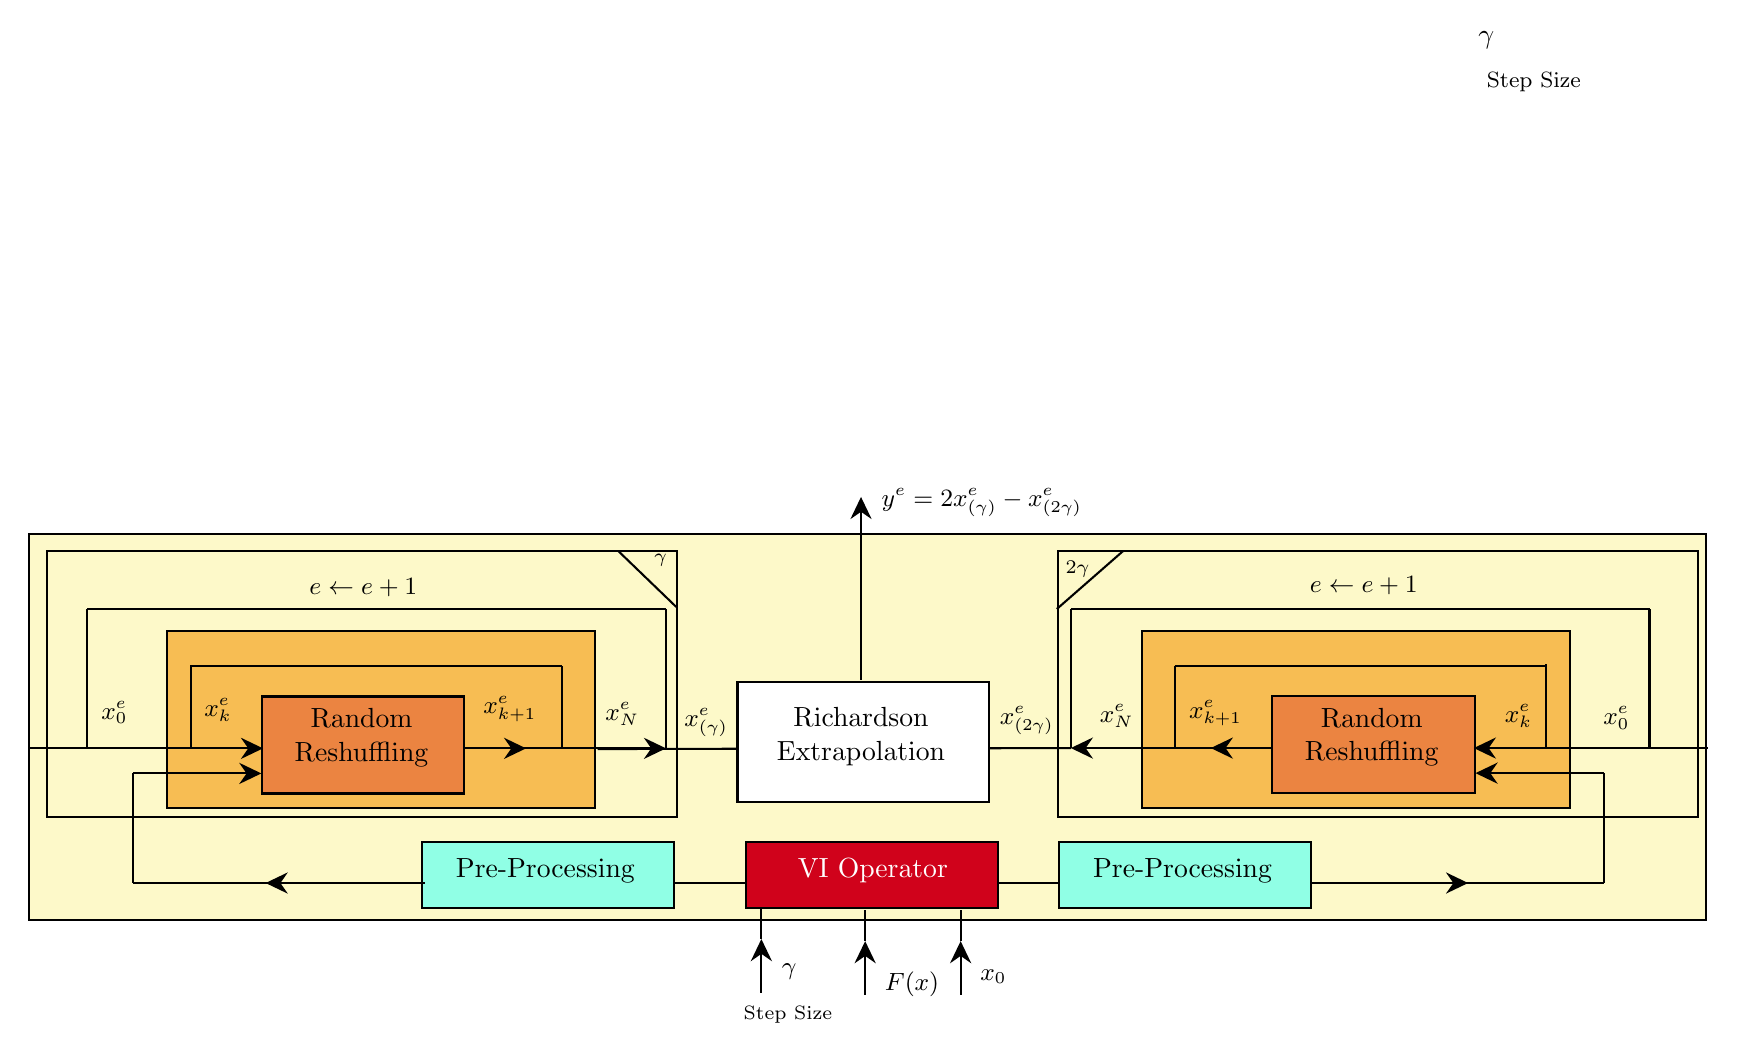
\begin{tikzpicture}[x=0.75pt,y=0.75pt,yscale=-1,xscale=1]
%uncomment if require: \path (0,711); %set diagram left start at 0, and has height of 711

%Shape: Rectangle [id:dp7167201570186642] 
\draw  [fill={rgb, 255:red, 248; green, 231; blue, 28 }  ,fill opacity=0.24 ] (24,362) -- (832,362) -- (832,548) -- (24,548) -- cycle ;
%Straight Lines [id:da5348252051360501] 
\draw    (215.16,530) -- (642,530) ;
%Straight Lines [id:da5870165356755055] 
\draw    (642,530) -- (783.02,530) ;
\draw [shift={(717.51,530)}, rotate = 180] [fill={rgb, 255:red, 0; green, 0; blue, 0 }  ][line width=0.08]  [draw opacity=0] (10.72,-5.15) -- (0,0) -- (10.72,5.15) -- (7.12,0) -- cycle    ;
%Shape: Rectangle [id:dp22967037843062987] 
\draw  [fill={rgb, 255:red, 245; green, 166; blue, 35 }  ,fill opacity=0.71 ] (90.45,408.54) -- (296.62,408.54) -- (296.62,493.84) -- (90.45,493.84) -- cycle ;
%Straight Lines [id:da17785199775015115] 
\draw    (74.14,477.2) -- (133.09,477.2) ;
\draw [shift={(136.09,477.2)}, rotate = 180] [fill={rgb, 255:red, 0; green, 0; blue, 0 }  ][line width=0.08]  [draw opacity=0] (10.72,-5.15) -- (0,0) -- (10.72,5.15) -- (7.12,0) -- cycle    ;
%Shape: Rectangle [id:dp2742561061453428] 
\draw  [fill={rgb, 255:red, 208; green, 2; blue, 27 }  ,fill opacity=0.3 ] (136.49,440.15) -- (233.94,440.15) -- (233.94,486.86) -- (136.49,486.86) -- cycle ;

%Straight Lines [id:da09921992906541832] 
\draw    (102.26,465.12) -- (133.9,465.12) ;
\draw [shift={(136.9,465.12)}, rotate = 180] [fill={rgb, 255:red, 0; green, 0; blue, 0 }  ][line width=0.08]  [draw opacity=0] (10.72,-5.15) -- (0,0) -- (10.72,5.15) -- (7.12,0) -- cycle    ;
%Straight Lines [id:da337709340044827] 
\draw    (234.35,465.12) -- (260.64,465.12) ;
\draw [shift={(263.64,465.12)}, rotate = 180] [fill={rgb, 255:red, 0; green, 0; blue, 0 }  ][line width=0.08]  [draw opacity=0] (10.72,-5.15) -- (0,0) -- (10.72,5.15) -- (7.12,0) -- cycle    ;
%Straight Lines [id:da8354383452527102] 
\draw    (240.28,465.12) -- (281.06,465.12) ;
%Straight Lines [id:da8152793732524597] 
\draw    (281.06,465.12) -- (281.06,425.65) ;
%Straight Lines [id:da7570544004782095] 
\draw    (102.26,465.12) -- (102.26,424.85) ;
%Straight Lines [id:da4721478714710243] 
\draw    (281.06,425.65) -- (102.26,425.65) ;
%Straight Lines [id:da3188806653380546] 
\draw    (281.06,465.12) -- (328.05,465.12) ;
\draw [shift={(331.05,465.12)}, rotate = 180] [fill={rgb, 255:red, 0; green, 0; blue, 0 }  ][line width=0.08]  [draw opacity=0] (10.72,-5.15) -- (0,0) -- (10.72,5.15) -- (7.12,0) -- cycle    ;
%Straight Lines [id:da5695989834818472] 
\draw    (52.27,465.12) -- (102.26,465.12) ;
%Straight Lines [id:da005449392824766197] 
\draw    (52.27,465.12) -- (52.27,398.2) ;
%Straight Lines [id:da5087383745711406] 
\draw    (331.05,465.12) -- (331.05,398.2) ;
%Straight Lines [id:da7805722702952284] 
\draw    (331.05,398.2) -- (52.27,398.2) ;
%Straight Lines [id:da42790020085683145] 
\draw    (52.27,465.12) -- (24.08,465.12) ;
%Shape: Rectangle [id:dp8867101993788168] 
\draw  [fill={rgb, 255:red, 245; green, 166; blue, 35 }  ,fill opacity=0.71 ] (766.71,408.41) -- (560.54,408.41) -- (560.54,493.71) -- (766.71,493.71) -- cycle ;
%Straight Lines [id:da45046936384949954] 
\draw    (783.02,477.06) -- (724.07,477.06) ;
\draw [shift={(721.07,477.06)}, rotate = 360] [fill={rgb, 255:red, 0; green, 0; blue, 0 }  ][line width=0.08]  [draw opacity=0] (10.72,-5.15) -- (0,0) -- (10.72,5.15) -- (7.12,0) -- cycle    ;
%Shape: Rectangle [id:dp8984113920591881] 
\draw  [fill={rgb, 255:red, 208; green, 2; blue, 27 }  ,fill opacity=0.3 ] (623.21,440.01) -- (720.67,440.01) -- (720.67,486.73) -- (623.21,486.73) -- cycle ;

%Straight Lines [id:da49889800256014705] 
\draw    (754.89,464.98) -- (723.26,464.98) ;
\draw [shift={(720.26,464.98)}, rotate = 360] [fill={rgb, 255:red, 0; green, 0; blue, 0 }  ][line width=0.08]  [draw opacity=0] (10.72,-5.15) -- (0,0) -- (10.72,5.15) -- (7.12,0) -- cycle    ;
%Straight Lines [id:da31365561028594713] 
\draw    (622.81,464.98) -- (596.52,464.98) ;
\draw [shift={(593.52,464.98)}, rotate = 360] [fill={rgb, 255:red, 0; green, 0; blue, 0 }  ][line width=0.08]  [draw opacity=0] (10.72,-5.15) -- (0,0) -- (10.72,5.15) -- (7.12,0) -- cycle    ;
%Straight Lines [id:da9666480403965403] 
\draw    (616.88,464.98) -- (576.1,464.98) ;
%Straight Lines [id:da6870758288531431] 
\draw    (576.1,464.98) -- (576.1,425.52) ;
%Straight Lines [id:da13859487218454614] 
\draw    (754.89,464.98) -- (754.89,424.71) ;
%Straight Lines [id:da30734305051591637] 
\draw    (576.1,425.52) -- (754.89,425.52) ;
%Straight Lines [id:da11442520008239165] 
\draw    (576.1,464.98) -- (529.1,464.98) ;
\draw [shift={(526.1,464.98)}, rotate = 360] [fill={rgb, 255:red, 0; green, 0; blue, 0 }  ][line width=0.08]  [draw opacity=0] (10.72,-5.15) -- (0,0) -- (10.72,5.15) -- (7.12,0) -- cycle    ;
%Straight Lines [id:da11238862430956253] 
\draw    (804.89,464.98) -- (754.89,464.98) ;
%Straight Lines [id:da3927723255927097] 
\draw    (804.89,464.98) -- (804.89,398.06) ;
%Straight Lines [id:da17493801390941033] 
\draw    (526.1,464.98) -- (526.1,398.06) ;
%Straight Lines [id:da38944767089549004] 
\draw    (526.1,398.06) -- (804.89,398.06) ;
%Straight Lines [id:da5789729604768556] 
\draw    (298.12,465.45) -- (526.1,464.98) ;
%Straight Lines [id:da5056140478751464] 
\draw    (804.89,464.98) -- (833.08,464.98) ;
%Shape: Rectangle [id:dp6283534568839406] 
\draw   (33,369.87) -- (336.12,369.87) -- (336.12,498) -- (33,498) -- cycle ;
%Straight Lines [id:da7766228141098565] 
\draw    (425,347) -- (425,432) ;
\draw [shift={(425,344)}, rotate = 90] [fill={rgb, 255:red, 0; green, 0; blue, 0 }  ][line width=0.08]  [draw opacity=0] (10.72,-5.15) -- (0,0) -- (10.72,5.15) -- (7.12,0) -- cycle    ;
%Shape: Rectangle [id:dp0677493839993355] 
\draw   (520.12,369.87) -- (828.12,369.87) -- (828.12,498) -- (520.12,498) -- cycle ;
%Shape: Rectangle [id:dp014110378228816445] 
\draw  [fill={rgb, 255:red, 255; green, 255; blue, 255 }  ,fill opacity=1 ] (365.5,433) -- (486.5,433) -- (486.5,491) -- (365.5,491) -- cycle ;

%Shape: Rectangle [id:dp8640505621986145] 
\draw  [fill={rgb, 255:red, 144; green, 255; blue, 229 }  ,fill opacity=1 ] (213.49,510.15) -- (335,510.15) -- (335,542) -- (213.49,542) -- cycle ;

%Shape: Rectangle [id:dp11807891437834184] 
\draw  [fill={rgb, 255:red, 144; green, 255; blue, 229 }  ,fill opacity=1 ] (520.49,510.15) -- (642,510.15) -- (642,542) -- (520.49,542) -- cycle ;

%Straight Lines [id:da6023255336667221] 
\draw    (74.14,477.2) -- (74.14,530) ;
%Straight Lines [id:da047541439752831094] 
\draw    (783.02,477.06) -- (783.02,529.87) ;
%Straight Lines [id:da38440122612945915] 
\draw    (74.14,530) -- (215.16,530) ;
\draw [shift={(138.15,530)}, rotate = 0] [fill={rgb, 255:red, 0; green, 0; blue, 0 }  ][line width=0.08]  [draw opacity=0] (10.72,-5.15) -- (0,0) -- (10.72,5.15) -- (7.12,0) -- cycle    ;
%Shape: Rectangle [id:dp7774128051215404] 
\draw  [fill={rgb, 255:red, 208; green, 2; blue, 27 }  ,fill opacity=1 ] (369.49,510.15) -- (491,510.15) -- (491,542) -- (369.49,542) -- cycle ;
%Straight Lines [id:da048020115234232885] 
\draw    (308,370) -- (336,397) ;
%Straight Lines [id:da22128359563915156] 
\draw    (551.33,370) -- (519.33,398) ;
%Straight Lines [id:da4178126076311651] 
\draw    (427,561) -- (427,584) ;
\draw [shift={(427,558)}, rotate = 90] [fill={rgb, 255:red, 0; green, 0; blue, 0 }  ][line width=0.08]  [draw opacity=0] (10.72,-5.15) -- (0,0) -- (10.72,5.15) -- (7.12,0) -- cycle    ;
%Straight Lines [id:da2712874934584891] 
\draw    (427,543) -- (427,558) ;
%Straight Lines [id:da22537158810197067] 
\draw    (377,560) -- (377,583) ;
\draw [shift={(377,557)}, rotate = 90] [fill={rgb, 255:red, 0; green, 0; blue, 0 }  ][line width=0.08]  [draw opacity=0] (10.72,-5.15) -- (0,0) -- (10.72,5.15) -- (7.12,0) -- cycle    ;
%Straight Lines [id:da17343167705220275] 
\draw    (377,542) -- (377,557) ;
%Straight Lines [id:da5797829827731849] 
\draw    (473,561) -- (473,584) ;
\draw [shift={(473,558)}, rotate = 90] [fill={rgb, 255:red, 0; green, 0; blue, 0 }  ][line width=0.08]  [draw opacity=0] (10.72,-5.15) -- (0,0) -- (10.72,5.15) -- (7.12,0) -- cycle    ;
%Straight Lines [id:da3209997322336591] 
\draw    (473,543) -- (473,558) ;

% Text Node
\draw (147.12,444.5) node [anchor=north west][inner sep=0.75pt]   [align=left] {\begin{minipage}[lt]{53.57pt}\setlength\topsep{0pt}
\begin{center}
Random \\Reshuffling
\end{center}

\end{minipage}};
% Text Node
\draw (382,444) node [anchor=north west][inner sep=0.75pt]   [align=left] {\begin{minipage}[lt]{62.26pt}\setlength\topsep{0pt}
\begin{center}
Richardson\\Extrapolation
\end{center}

\end{minipage}};
% Text Node
\draw (721,118.4) node [anchor=north west][inner sep=0.75pt]    {$\gamma $};
% Text Node
\draw (725,138) node [anchor=north west][inner sep=0.75pt]  [font=\footnotesize] [align=left] {Step Size\\};
% Text Node
\draw (633.84,444.37) node [anchor=north west][inner sep=0.75pt]   [align=left] {\begin{minipage}[lt]{53.57pt}\setlength\topsep{0pt}
\begin{center}
Random \\Reshuffling
\end{center}

\end{minipage}};
% Text Node
\draw (107.08,439.73) node [anchor=north west][inner sep=0.75pt]  [font=\small]  {$x_{k}^{e}$};
% Text Node
\draw (241.59,438.5) node [anchor=north west][inner sep=0.75pt]  [font=\small]  {$x_{k+1}^{e}$};
% Text Node
\draw (300.38,441.53) node [anchor=north west][inner sep=0.75pt]  [font=\small]  {$x_{N}^{e}$};
% Text Node
\draw (57.55,441.12) node [anchor=north west][inner sep=0.75pt]  [font=\small]  {$x_{0}^{e}$};
% Text Node
\draw (157.77,381.59) node [anchor=north west][inner sep=0.75pt]  [font=\small]  {$e\leftarrow e+1$};
% Text Node
\draw (522.12,373.27) node [anchor=north west][inner sep=0.75pt]  [font=\scriptsize]  {$2\gamma $};
% Text Node
\draw (581.57,440.59) node [anchor=north west][inner sep=0.75pt]  [font=\small]  {$x_{k+1}^{e}$};
% Text Node
\draw (733.67,442.41) node [anchor=north west][inner sep=0.75pt]  [font=\small]  {$x_{k}^{e}$};
% Text Node
\draw (538.59,442.4) node [anchor=north west][inner sep=0.75pt]  [font=\small]  {$x_{N}^{e}$};
% Text Node
\draw (781.21,443.59) node [anchor=north west][inner sep=0.75pt]  [font=\small]  {$x_{0}^{e}$};
% Text Node
\draw (433.38,338.53) node [anchor=north west][inner sep=0.75pt]  [font=\small]  {$y^{e} =2x_{( \gamma )}^{e} -x_{( 2\gamma )}^{e}$};
% Text Node
\draw (639.77,380.59) node [anchor=north west][inner sep=0.75pt]  [font=\small]  {$e\leftarrow e+1$};
% Text Node
\draw (338.38,444.53) node [anchor=north west][inner sep=0.75pt]  [font=\small]  {$x_{( \gamma )}^{e}$};
% Text Node
\draw (490.38,443.53) node [anchor=north west][inner sep=0.75pt]  [font=\small]  {$x_{( 2\gamma )}^{e}$};
% Text Node
\draw (223.12,516.5) node [anchor=north west][inner sep=0.75pt]   [align=left] {\begin{minipage}[lt]{72.45pt}\setlength\topsep{0pt}
\begin{center}
Pre-Processing
\end{center}

\end{minipage}};
% Text Node
\draw (323.83,369.96) node [anchor=north west][inner sep=0.75pt]  [font=\scriptsize]  {$\gamma $};
% Text Node
\draw (530.12,516.5) node [anchor=north west][inner sep=0.75pt]   [align=left] {\begin{minipage}[lt]{72.45pt}\setlength\topsep{0pt}
\begin{center}
Pre-Processing
\end{center}

\end{minipage}};
% Text Node
\draw (382.12,516.5) node [anchor=north west][inner sep=0.75pt]  [color={rgb, 255:red, 255; green, 255; blue, 255 }  ,opacity=1 ] [align=left] {\begin{minipage}[lt]{63.95pt}\setlength\topsep{0pt}
\begin{center}
 \ \ VI Operator
\end{center}

\end{minipage}};
% Text Node
\draw (435,571.4) node [anchor=north west][inner sep=0.75pt]  [font=\small]  {$F( x)$};
% Text Node
\draw (385.38,567.53) node [anchor=north west][inner sep=0.75pt]  [font=\small]  {$\gamma $};
% Text Node
\draw (367,588) node [anchor=north west][inner sep=0.75pt]  [font=\scriptsize] [align=left] {Step Size};
% Text Node
\draw (481,570.4) node [anchor=north west][inner sep=0.75pt]  [font=\small]  {$x_{0}$};


\end{tikzpicture}
}
%%%%%%%%   % \caption{Algorithmic Model of \RRresh$\oplus$\RRrom}
%%%%%%%%\end{figure}
%%%%
%%%%This synthesis of reshuffling with Richardson extrapolation not only closes a gap in the theoretical landscape, but also delivers a sharp punchline: **bias rates previously thought to plateau at $\mathcal{O}(\gamma^2)$ can be further reduced to $\mathcal{O}(\gamma^3)$ through principled composition of these heuristics.** We view this as a stepping stone toward a more general theory of bias reduction in stochastic variational inequalities.
%%%%
%%%%
%%%%
%%%%
%%%%%To obtain our main result we devise a more general principled framework that can be applied to many other variations of stochastic gradient methods constant step-sizes. like  single-call or multi-call stochastic extra-gradient methods \cite{?}, like extra-gradient\cite{?}, optimistic\cite{?}, mirror-prox\cite{?} , αλλα αφηνουμε την περαιτερω μελετη σε future work beyond scope of the paper. Our framework splits the design problem into two steps, the algorithmic design and the asymptotic analysis of the probabilistic nature of our algorithm.\\
%%%%%\textbf{Our algorithm.} 
%%%%%Υπάρχουν πολύ τρόποι να συνδιαστει το \RRrom kai \RRresh intra or inter epoch και με διαφορετικη σειρα. Εμεις επιλεγουμε τον πιο φυσικο που συμβαινει στην πραξη αφου το \RRrom χρησιμοποιειται συχνα ως final step σε black-box συστηματα in a higher level και επιτρεπει την παραλληλοποιηση του αλγοριθμου ενω \RRresh ειναι core επιλογη για το low-level training. Ετσι, 
%%%%%We analyze stochastic gradient algorithms that use random reshuffling as the sampling technique for selecting the data and estimating the stochastic oracles of the gradients/operators at them. Specifically, at the start of each epoch $k >0$ a permutation $\omega_k$ of $[n]$ is drawn uniformly at random, specifying an ordering of the data in the dataset for evaluating the stochastic gradients inside the epoch. The algorithm consequently performs the classical update rule of SGD\footnote{Στην min-max optimization ο αλγοριθμος αναφερεται ως sgda, αφου επικρατει το zero-sum two-player utility perspective and o ενας πεφτει και ο αλλος μεγαλωνει (See Section~\textcolor{red}{X})} 
%%%%%\begin{equation}\tag{SGD-\RRrom$\oplus$\RRresh (in)}
%%%%%    x_k^{i+1} = x_k^i - \gamma PreProcess[\mathrm{StochOracle}[grad/VI-operator](x^i_k; \omega_k^i)] \label{SGD-4R1}
%%%%%\end{equation}
%%%%%$g(x_i^k; \omega_k^i)$ is the stochastic oracle evaluated at $x^i_k$ ειτε το gradient of loss for minimization case or $F_{\omega_k^i}(x_k^i)$ στην γενικη περιπτωση του VI operator and defined by the corresponding $\omega_k^i$ data point of the dataset.
%%%%%Ταυτόχρονα όμως θα πρέπει να αντιμετωπίσουμε μια ιδιαιτερότητα του \RRresh: Όταν ολοκληρωθεί ο υπολογισμός του epoch και parse online all data, the corresponding cumulative grad stimator ως τυχαια μεταβλητη ειναι biased του gradient estimator του finite-sum (αυτος ειναι και ο βασικος λογος που η vast majority of literature leverages with replacement αφου κανει τις αποδειξεις technically easier). Επισης η φυση του θορυβου ειναι διακριτος αφου στηριζεται στο permutation και το support ειναι διακριτο. Για να αντιμετωπισουμε καθως τα θεωρητικα αποτελεσματα \RRrom εφαρμογεται σε stochastic optimization (assuming continuous distribution or infinite dataset) χρησιμοποιουμε ενα PreProcess routine. 
%%%%% To inguine κομματι ειναι το support του θορυβου να ομαλοποιηθει, επιτρεποντας το toolbox \RRrom, αλλα απο την αλλη rate of convergence and moments of noise να παραμεινουν ιδιας ταξης με αυτη χωρις την παρουσια του θορυβου Στην περίπτωση μας δείχνουμε ενα perturbation με ένα gaussian noise με well-tailored lower scale variance αρκεί. Αν και στην πράξη το μεγεθος των δεδομενων ειναι αρκετο ωστε να γεφυρωνεται αυτο το χασμα απο μονο του, we conjecture οτι μπορει να γινει avoid.
%%%%% Τέλος στο τέλος κάθε epoch, εφαρμόζουμε \RRrom
%%%%% \begin{equation}\tag{SGD-\RRrom$\oplus$\RRresh (out)}
%%%%%    \hat{x}_Ν^{i+1} = 2x_{Ν,(\gamma)}^i - x_{Ν,(2\gamma)}\label{SGD-4R2}
%%%%%\end{equation}
%%%%
%%%%\newpage
%%%%
%%%%\textit{Paragraph on the Algorithm} We analyze stochastic gradient algorithms that use random reshuffling as the sampling technique for selecting the data and estimating the stochastic oracles of the gradients/operators at them. Specifically, at the start of each epoch $k >0$ a permutation $\omega_k$ of $[n]$ is drawn uniformly at random, specifying an ordering of the data in the dataset for evaluating the stochastic gradients inside the epoch. The algorithm consequently performs the classical update rule of SGD(A) 
%%%%\begin{equation}\tag{SGDA-RR}
%%%%    x_k^{i+1} = x_k^i - \gamma g(x^i_k; \omega_k^i) \label{SGDA-RR}
%%%%\end{equation}
%%%%where $g(x_i^k; \omega_k^i)$ is the stochastic oracle evaluated at $x^i_k$ and defined by the corresponding $\omega_k^i$ data point of the dataset. In this work, we allow the stochastic oracle to be either the typical stochastic gradient $g(x_i^k; \omega_k^i) = F_{\omega_k^i}(x_k^i)$ or a smooth version of it [motivated by applications and cite papers here]. 
%%%%As a last step, the last iterate of the epoch is set as a starting point for the next epoch and the algorithm reiterates. 
%%%%
%%%%
%%%%\section{Long-Run Distribution of SGD}
%%%%
%%%%Our goal in this part is to quantify the long-run distribution of SGD in the most general manner possible. To do so, we take an approach based on the theory of large deviations \cite{dembo1998} and randomly perturbed dynamical systems \cite{freidlin2012, kifer1981}, which enables us to estimate the probability of ``rare events'' (such as $x_n$ moving against the gradient flow of $f$ for a protracted period of time). 
%%%%
%%%%This allows us to characterize the events that occur with high probability and establish the following hierarchy of results:
%%%%
%%%%\begin{enumerate}
%%%%    \item In the long run, the critical region of $f$ is visited exponentially more often than any non-critical region.
%%%%    \item The iterates of SGD are concentrated with exponentially high probability in the vicinity of a region that minimizes a certain energy functional which depends on $f$ and the statistics of the noise. Importantly, the ground state of this functional does not necessarily coincide with the global minimum of $f$.
%%%%    \item Among the remaining connected components of critical points, each component is visited with frequency which is exponentially proportional to its energy, according to the Boltzmann--Gibbs distribution of statistical physics with temperature equal to the method’s step-size.
%%%%    \item Every connected component of non-minimizing critical points of $f$—i.e., local maximizers or saddle points—is dominated by a component of local minimizers that is visited exponentially more often.
%%%%\end{enumerate}
%%%%
%%%%Finally, we derive an explicit characterization of the invariant measure of SGD under Gaussian noise and other noise models motivated by deep learning considerations. Taken together, these properties resemble those of a canonical ensemble in statistical physics: in a sense, each connected component of critical points can be seen as a ``state'' of a statistical ensemble, and the step-size of SGD plays the role of the system’s (fixed) temperature.
%%%%
%%%%\section{General Framework for Private Estimation}
%%%%
%%%%To obtain our main result we devise a more general principled framework that can be applied to many other problems in private statistical estimation. Our framework splits the design problem into two steps, inspired by earlier work on learning Erdős--Rényi graphs and graphons \cite{BCSZ18a, BCSZ18c}:
%%%%
%%%%\begin{enumerate}
%%%%    \item We obtain private algorithms for a subset of the domain, focusing attention on a restricted class of instances that are typical with respect to the distribution. We define constraints that samples satisfy with high probability and focus only on instances that meet those constraints. In this restricted setting, we obtain an estimator that is accurate and private.
%%%%    \item We extend our estimator to all instances and guarantee privacy globally. We employ a method for Lipschitz extensions---the ``Extension Lemma'' from \cite{BCSZ18a}---which allows extending a private algorithm from a smaller domain $A$ to a larger domain $B$ without changing the output distribution for instances in $A$, while only worsening privacy guarantees by a factor of~2.
%%%%\end{enumerate}
%%%%
%%%%Finally, we show that this extension can be computed in polynomial time by characterizing the structure of the resulting extended output distributions, showing they are piece-wise constant or exponential with polynomially many pieces. We identify all pieces through a greedy algorithm and sample exactly from the resulting distribution. This provides the first instance of a natural problem for which the extension lemma can be computed in polynomial time.
%%%%
%%%%
%%%%
%%%%
%%%%

%To the best of our knowledge, this work is the first to demonstrate that these heuristics can be synthesized into a principled algorithmic framework, yielding a composite bias reduction unattainable by any of them in isolation.



% Concretely, whenever the bias expands as $\text{bias}_{}(\gamma) = \Delta \gamma + \mathcal{O}(\gamma^{\kappa})$ for some $\kappa>1$,
% then if 
%         $x_{\infty}^{\gamma} - x^* = \Delta\dot\gamma + \mathcal{O}(\gamma^{\kappa}), \quad x_{\infty}^{2\gamma} - x^* = \Delta\dot 2\gamma + \mathcal{O}(\gamma^{\kappa})$ then extrapolating yields
% $        2x_{\infty}^{\gamma}- x_{\infty}^{2\gamma} - x^* = \cancel{2\Delta \gamma} - \cancel{2\Delta \gamma} + \mathcal{O}\left(\gamma^{\kappa}\right) = \mathcal{O}\left(\gamma^{\kappa}\right) \nonumber
% $

% \begin{eqnarray}
%         x_{\infty}^{\gamma} - x^* = \Delta\dot\gamma + \mathcal{O}(\gamma^{\kappa}), \quad x_{\infty}^{2\gamma} - x^* = \Delta\dot 2\gamma + \mathcal{O}(\gamma^{\kappa})\\
%         2x_{\infty}^{\gamma}- x_{\infty}^{2\gamma} - x^* = \cancel{2\Delta \gamma} - \cancel{2\Delta \gamma} + \mathcal{O}\left(\gamma^{\kappa}\right) = \mathcal{O}\left(\gamma^{\kappa}\right) \nonumber
% \end{eqnarray}

% \newpage

% Orthogonal to the above, another classical debiasing technique has recently gained traction in stochastic optimization: Richardson–Romberg (RR) extrapolation. Originally developed in numerical analysis to improve the accuracy of discretization schemes [Hildebrand, 1987], RR operates by combining approximations with different step sizes so as to cancel the leading term in the error expansion. The one-step version was introduced to reduce discretization error in Euler schemes for stochastic differential equations [Talay & Tubaro, 1990], later extended to non-smooth settings [Bally & Talay, 1996] and multistep discretizations [Pages, 2007].

% The same idea can be applied to constant-step stochastic gradient methods: if the stationary bias admits an expansion of the form
% x_{\infty}^{\gamma} - x^* = \Delta \gamma + \mathcal{O}(\gamma^{\kappa}),
% \quad
% x_{\infty}^{2\gamma} - x^* = 2\Delta \gamma + \mathcal{O}(\gamma^{\kappa}),
% then extrapolating yields
% 2x_{\infty}^{\gamma} - x_{\infty}^{2\gamma} - x^*
% = \cancel{2\Delta \gamma} - \cancel{2\Delta \gamma} + \mathcal{O}(\gamma^{\kappa})
% = \mathcal{O}(\gamma^{\kappa}),
% thereby eliminating the dominant bias term. This simple yet powerful idea has motivated a growing line of work applying RR to stochastic approximation methods, including SGD [Durmus et al., 2016; Dieuleveut et al., 2020; Merad & Gaïffas, 2023; Huo et al., 2024a], Q-learning, and other single- and two-timescale algorithms [Allmeier & Gast, 2024; Zhang & Xie, 2024; Huo et al., 2024a; Kwon et al., 2024].

% Despite this progress, the theoretical understanding of RR in the context of stochastic VIs remains nascent. Prior work has either assumed unbiased stochastic oracles [Bach], or leveraged specific structural properties of the noise [Vlatakis et al.]. Thus, while RR has proven effective in practice and across related stochastic approximation problems, its guarantees for general variational inequalities are still incomplete.

% \newpage


% Orthogonal to the above, there is another folkore from numerical analysis debiasing technique that has become popular in the field of stochastic VIs, the Richardson - Romberg extrapolation. Richardson requires a more refined analysis of the bias of the method, decomposing into a dominant term and some higher order ones, resulting in $\text{bias}_{}(\gamma) = \Delta \gamma + \mathcal{O}(\gamma^{\kappa})$
% \begin{eqnarray}
%         x_{\infty}^{\gamma} - x^* = \Delta\dot\gamma + \mathcal{O}(\gamma^{\kappa}), \quad x_{\infty}^{2\gamma} - x^* = \Delta\dot 2\gamma + \mathcal{O}(\gamma^{\kappa})\\
%         2x_{\infty}^{\gamma}- x_{\infty}^{2\gamma} - x^* = \cancel{2\Delta \gamma} - \cancel{2\Delta \gamma} + \mathcal{O}\left(\gamma^{\kappa}\right) = \mathcal{O}\left(\gamma^{\kappa}\right) \nonumber
% \end{eqnarray}
% Despite the simplicity of the method, the theoretical understanding is nascent. Papers for Richardson explaining the method in minimization (cite Bach) and in VI (Vlatakis). The first analyzed the method with unbiased stochastic oracles, while the second were utilizing specific structure of the noise. 

% Richardson-Romberg (RR) extrapolation is a technique used to improve the accuracy of numerical approximations (Hildebrand, 1987), such as those from numerical differentiation or integration. It involves using approximations with different step sizes and then extrapolating to reduce the error, typically by removing the leading term in the error expansion. The one-step RR extrapolation was introduced to reduce the discretization error induced by an Euler scheme to simulate stochastic differential equation in Talay & Tubaro (1990), and later generalized for non-smooth functions in Bally & Talay (1996). This technique was extended using multistep discretizations in Page`s (2007). RR extrapolation have been applied to Stochastic Gradient Descent (SGD) methods in Durmus et al. (2016), Dieuleveut et al. (2020), Merad & Ga ̈ıffas (2023) and Huo et al. (2024a), to improve convergence and reduce error in optimization problems, particularly when dealing with noisy or high-variance gradient estimates. Recent papers (Allmeier & Gast, 2024; Zhang & Xie, 2024; Huo et al., 2024a; Kwon et al., 2024) consider applications of RR to different stochastic approximation problems with constant step-size, including Q-learning, and single- and two-timescale stochastic approximation.


% To address this issue, practitioners often turn to debiasing heuristics. One such technique, widely adopted in stochastic optimization, is \emph{random reshuffling} (RR), or \emph{without-replacement} sampling, where each data point is used exactly once per epoch. Unlike the classical \emph{with-replacement} variant of SGD—where samples are drawn independently and some may be revisited while others are skipped. RR eliminates this redundancy by enforcing a full pass over the dataset in a random order, closely matching how large-scale training is implemented in practice.
% Despite the dependence it induces across samples within an epoch, recent work has established faster convergence guarantees for RR in both minimization and VIPs \cite{Ahn et al., 2020; Gürbüzbalaban et al., 2021; Mishchenko et al., 2020a; Cai et al., 2023}. Beyond these rate improvements, RR has also been shown to reduce the stationary bias of constant-step methods from $\mathcal{O}(\gamma)$ to $\mathcal{O}(\gamma^2)$ under suitable conditions.

%To address this issue, practitioners often turn to debiasing heuristics. One such technique, widely adopted in stochastic optimization, is \emph{random reshuffling} (RR)\textendash also known as \emph{without-replacement}, which samples each data point exactly once per epoch. In contrast, the classical \emph{with-replacement} variant of SGD draws each sample independently at every step, so the same data point may be visited multiple times while others are skipped. RR eliminates this redundancy by enforcing a full pass over the dataset in a random order, a procedure that aligns closely with how practitioners typically implement large-scale training, owing to its ease of use and superior empirical performance \cite{Bottou, 2012}. Despite the additional technical challenges introduced by the dependence across samples within an epoch, a series of recent works has established faster convergence guarantees for RR across minimization and variational inequality problems \cite{Ahn et al., 2020; Gürbüzbalaban et al., 2021; Mishchenko et al., 2020a; Cai et al., 2023}. Strikingly, beyond rate improvements, reshuffling has also been shown to mitigate the stationary bias of constant-step stochastic methods, sharpening it from $\mathcal{O}(\gamma)$ down to $\mathcal{O}(\gamma^2)$ under suitable conditions.

% For example, a particularly important design choice is the use of a \emph{constant step size}. In practice, this setting is extremely popular: it makes the algorithm easy to tune, quickly erases dependence on initialization, and yields rapid early progress \cite{?,?}. Yet it comes with a fundamental limitation: convergence stalls at a non-vanishing bias. Even in the simple case of strongly convex problems with a unique solution $x^$, one typically has
% $\|x_k - x_*\|^2 \;=\; e^{-\rho k}\|x_0 - x_*\|^2 \;+\; \text{bias}(\gamma),$
% with $\text{bias}(\gamma) = \mathcal{O}(\gamma)$. Thus, in the long run, the iterates stabilize at a point whose distance from the optimum is of order $\gamma$.
% To facilitate analysis, the leitmotif of the community
% isolates one of these design choices while holding the rest fixed — a ceteris paribus approach that yields valuable but fragmented insights into their impact.
% examines these choices in isolation—adopting a ceteris paribus perspective that clarifies their individual impact but obscures their interaction.



% In practice, many of these tasks reduce to finite-sum formulations, where the objective depends on a large collection of data samples or agents. The success of modern large-scale learning hinges on stochastic methods, which overcome the prohibitive cost of computing full gradients by sampling and updating with only a few components at each iteration.


% Variational inequalities (VIs) form a unifying framework for a wide range of machine learning problems, including adversarial robustness, reinforcement learning, and min–max optimization.




% What is the problem?
% Why the problem is important?
% Why the problem is unsolved/history 
% How we resolve it
% Why it was not trivial?


% VI's are important + applications

% Finite-sum: success of Stochastic gradient methods to tame the lack of full-gradient. 
% In the last decades, there is a great effort from the theory community to explain the heuristics that tune the performance of the method in practice.

% The community has explored the effects of an algorithmic heuristic isolated and not the synergy with other common ones. 

% Constant step size: in practice it is used but this leads to bias remaining
% \begin{eqnarray}
%     \|x_k - x_*\|^2 &=& \exp{-\rho k} \|x_0 - x_*\|^2 + \text{bias}(\gamma) \nonumber
% \end{eqnarray}
% The bias in SGD is $\text{bias}(\gamma) = \mathcal{O}(\gamma)$. The limit of the iterates could be off the optimal value by a magnitude of order $\text{bias}(\gamma)$. 

% In practice, RR is used because it is beneficial (cite papers). Recently found they provide debiasing $\text{bias}_{\text{RR}}(\gamma) = \mathcal{O}(\gamma^2)$.

% Orthogonal to the above, there is another folkore from numerical analysis debiasing technique that has become popular in the field of stochastic VIs, the Richardson - Romberg extrapolation. Richardson requires a more refined analysis of the bias of the method, decomposing into a dominant term and some higher order ones, resulting in $\text{bias}_{}(\gamma) = \Delta \gamma + \mathcal{O}(\gamma^{\kappa})$
% \begin{eqnarray}
%         x_{\infty}^{\gamma} - x^* = \Delta\dot\gamma + \mathcal{O}(\gamma^{\kappa}), \quad x_{\infty}^{2\gamma} - x^* = \Delta\dot 2\gamma + \mathcal{O}(\gamma^{\kappa})\\
%         2x_{\infty}^{\gamma}- x_{\infty}^{2\gamma} - x^* = 2 \Delta\dot\gamma - 2\Delta\dot\gamma + \mathcal{O}\left(\gamma^{\kappa}\right) = \mathcal{O}\left(\gamma^{\kappa}\right) \nonumber
% \end{eqnarray}

% Despite the simplicity of the method, the theoretical understanding is nascent. Papers for Richardson explaining the method in minimization (cite Bach) and in VI (Vlatakis). The first analyzed the method with unbiased stochastic oracles, while the second were utilizing specific structure of the noise. 

% In this work, we ask the question: 
% What is the mutual impact of all the aforementioned heuristics when they are applied simultaneously?

% This questions makes sense and it is non-trivial, as the RR heuristic provides a biased stochastic oracle. Even if Emmanouilidis et al. provide bounds in the second moment, the noise from the stochastic algorithm is discrete and thus direct application of the previous results (Bach, Vlatakis) do not hold. In this work, it is the first time to the best of our knowledge that we present an algorithmic way to combine the heuristics in an effective way for reducing the bias in a composite way. 

% Figure with both plots (left: bias vs step-size, right: 2D plot showing neighbourhoods)

% Algorithm: legend provide details about smoothing noise

 
 
%%%%%
%%%%%\textit{Paragraph on the Algorithm} We analyze stochastic gradient algorithms that use random reshuffling as the sampling technique for selecting the data and estimating the stochastic oracles of the gradients/operators at them. Specifically, at the start of each epoch $k >0$ a permutation $\omega_k$ of $[n]$ is drawn uniformly at random, specifying an ordering of the data in the dataset for evaluating the stochastic gradients inside the epoch. The algorithm consequently performs the classical update rule of SGD(A) 
%%%%%\begin{equation}\tag{SGDA-RR}
%%%%%    x_k^{i+1} = x_k^i - \gamma g(x^i_k; \omega_k^i) \label{SGDA-RR}
%%%%%\end{equation}
%%%%%where $g(x_i^k; \omega_k^i)$ is the stochastic oracle evaluated at $x^i_k$ and defined by the corresponding $\omega_k^i$ data point of the dataset. In this work, we allow the stochastic oracle to be either the typical stochastic gradient $g(x_i^k; \omega_k^i) = F_{\omega_k^i}(x_k^i)$ or a smooth version of it [motivated by applications and cite papers here]. 
%%%%%As a last step, the last iterate of the epoch is set as a starting point for the next epoch and the algorithm reiterates. 
